% !TEX program = xelatex
% !TEX encoding = UTF-8 Unicode
% !Mode:: "TeX:UTF-8"

\documentclass[openany]{ctexbook}
\usepackage{ctex}  
\usepackage{tikz}
\usepackage{geometry}
\usepackage{pdfpages} %将PDF文件加入到封面位置
\geometry{a4paper,left=1.5cm,right=1.5cm,top=3cm,bottom=3cm}
\usepackage{hyperref}
\usepackage{amsmath}
\usepackage{xcolor}
\usepackage[utf8]{inputenc}
\usepackage{graphicx}
\usepackage{fancyhdr}
\usepackage{listings}
\usepackage{array}
\usepackage{tikz}
\usepackage[title]{appendix}
\usetikzlibrary{arrows.meta,
	positioning,
	quotes}
\usepackage[figuresright]{rotating}

% Define color
\definecolor{vivadodraw}{rgb}{0.2549,0.3804,0.6235}
\definecolor{vivadofill}{rgb}{0.9294,0.9647,0.9960}

\lstset{
 columns=fixed,       
 numbers=left,                                        % 在左侧显示行号
 numberstyle=\tiny\color{gray},                       % 设定行号格式
 frame=none,                                          % 不显示背景边框
 backgroundcolor=\color[RGB]{245,245,244},            % 设定背景颜色
 keywordstyle=\color[RGB]{40,40,255},                 % 设定关键字颜色
 numberstyle=\footnotesize\color{darkgray},           
 commentstyle=\it\color[RGB]{0,96,96},                % 设置代码注释的格式
 stringstyle=\ttfamily\color[RGB]{128,0,0},   % 设置字符串格式
 showstringspaces=false,                              % 不显示字符串中的空格
 language=c,                                        % 设置语言
}


\begin{document}  

\begin{titlepage}	
% 封面信息

\includepdf[pages={1}]{cover.pdf} %曲线救国的思路,外界自建封面,然后调用
\end{titlepage}

\tableofcontents

\let\cleardoublepage\clearpage % 去空白

\mainmatter
% Part 1 概述
\chapter{概述}

\section{项目背景}

马家沟河(Ma-River)是第七届”龙芯杯“全国大学生计算机系统能力培养大赛(NSCSCC 2023)的参赛作品。

项目实现了基于MIPS32 Release1指令集的多发射乱序处理器软核——Ma-River CPU,并在此基础上自行构建了SoC,自行设计实现了多个外设控制器,可以运行U-Boot、ucore、Linux,并为其移植或自行实现了大量丰富应用,实现了一个完整的基于FPGA的嵌入式计算机系统。

\section{项目概述}

\subsection{设计模式}

Ma-River的所有硬件设计使用Verilog HDL实现。

在项目前期的结构设计阶段,我们使用C++编写了模拟CPU结构的周期精确模拟器,根据其在benchmark上的性能表现,进行精确的结构调整,使我们以极低代价得到具有优秀IPC的精简结构设计方案。后期直接据此进行RTL实现。

在项目后期的调试阶段,我们自行实现了指令自动生成器,可以根据不同场景生成大量随机指令,通过trace比对尽可能消除CPU核的潜在bug。

\subsection{CPU架构}

Ma-River CPU是六发射超标量乱序处理器,支持128条MIPS32 Release1指令。主流水线11级,取指/提交宽度为2,后端具有用于指令执行的4个整数功能单元和2个浮点功能单元,每周期最多发射执行6条指令。处理器核在整体上分为整数和浮点两个相对独立的部分,二者共享取指/访存/ROB/提交部件。

Ma-River CPU正确实现了CP0、TLB、精确异常等系统支持所需部件,能够支持Linux等操作系统的正常启动运行。

\subsection{SoC设计}
为了充分利用实验箱上的提供的丰富外设、发挥CPU核的性能,我们基于Vivado Block Design设计了一套功能较完备的SoC。我们通过自行设计的控制器和已有的IP核,能够操作板上的绝大多数功能模块,包括:

- VGA:控制器自行实现;分辨率1024*768,支持字符和图像模式;支持DMA,适配了Framebuffer驱动

- LCD:控制器自行实现;分辨率480*800,支持字符和图像模式;支持DMA,适配了Framebuffer驱动

- LCD触摸:使用AXI IIC IP核实现,并使用自行实现的模块进行硬复位

- PS/2:控制器自行实现;支持PS/2键盘输入

- GPIO:控制器自行实现;支持以中断方式获取按键状态,支持控制LED、数码管

- DRAM:使用Xilinx MIG 7 Series IP核实现

- 串口:使用AXI UART16550 IP核实现

- 以太网:使用AXI Ethernetlite IP核实现

同时,我们通过拓展I/O接口,可对板外SD卡进行读写操作。


\subsection{系统软件}

Ma-River使用U-Boot进行引导,可以启动ucore和Linux(最新的6.4版本)操作系统。在Linux上,我们自行实现和移植了VGA Console、LCD、FrameBuffer、键盘等驱动程序,并且还实现了Linux终端的中文输入输出支持。

我们为Linux移植了buildroot,通过网口挂载NFS文件系统,并在此基础上移植了GCC、Python、QEMU等软件,自行编写或移植了LVGL GUI、Gif动画播放器、3D实时渲染器等图形应用。
% Part 2 CPU
\chapter{CPU}

\section{概述}

\begin{description}

\item[指令集] \quad Ma-River CPU实现了MIPS32 Release1的一个较完整子集,包括全部的算术逻辑指令、分支跳转指令(包括likely)、陷阱指令、访存指令、浮点运算指令(CP1)、大部分特权指令(perf和sync实现为nop),共128条。

\item[整体架构] \quad Ma-River CPU是取指/提交宽度为2的六发射超标量乱序处理器,分为整数和浮点(FPU)两个相对独立的部分,这两个部分共享取指部件和ROB(32表项)。整数部分的主流水线共11级,可大致划分为分支预测、取指(两级)、译码、寄存器重命名、分发、发射、执行、写回ROB、提交(两级)。执行阶段具有4个并行工作的功能单元:ALU0/1(单周期,执行大部分算术逻辑指令)、访存(AGU+LSU,两级流水,执行访存指令)、MDU(多周期,执行乘除指令及其它杂项指令)。FPU部分具有译码、寄存器重命名、分发、发射、执行(多周期,两个功能单元)、写回ROB的流水段,取指后的指令在经过第一个译码阶段后可被送入FPU,运算结果写回ROB后与CPU指令统一提交。

\item[CP0与异常] \quad 为完成大赛要求并正确启动Linux操作系统,Ma-River CPU实现了18个CP0寄存器(包括Release 2定义的EBase),并正确实现了12种异常的精确支持。

\item[Cache] \quad Ma-River CPU实现了4KB$\times$4路的i-Cache和4KB$\times$3路的d-Cache,均为两级流水访问,并正确实现了Cache维护指令。为提升性能,d-Cache还具备1个Outstanding miss支持以及修改可动态回滚的特性。

\item[TLB MMU] \quad Ma-River CPU实现了具有64个表项的TLB,并正确实现了全部TLB维护指令及异常,支持4KB$\sim$256MB的动态页面大小配置(通过CP0.PageMask实现)。我们将TLB设计为对体系结构隐藏的两级分立结构,作为缓存的L1 i-TLB和d-TLB各具有3个表项。

\item[分支预测] \quad Ma-River CPU的分支预测主要采取基于指令局部分支历史的BTB(256个表项)+LHT(12位历史)的方式,此外对于函数返回指令使用容量为4的RAS硬件栈额外进行预测。

\item[FPU] \quad Ma-River CPU正确实现了MIPS32 Release1定义的全部30条支持单精度/双精度/定点数据类型运算的浮点指令。我们自行设计实现了用于浮点加法、乘法、除法、平方根、取整、转换操作的动态多功能流水线运算部件,无需使用专用IP。

\item[性能] \quad Ma-River能够以118MHz的频率在大赛的性能测试中取得高达110.50的性能成绩,相对GS132的平均IPC比达到46.71。Linpack测得浮点算力达3.23MFLOPS。

\end{description}

\section{流水线结构}

Ma-River CPU的整体结构见图2.1,下面对主要流水段进行简要说明:

\begin{sidewaysfigure}[htbp]
    \centering
    \begin{tikzpicture}[scale=0.95]
        %\draw [loosely dashed] (0,0)--(0,10); %较疏的线状虚线
        %\draw [loosely dashed] (5,0)--(5,10); %较疏的线状虚线
        %\draw [loosely dashed] (10,0)--(10,10); %较疏的线状虚线
        %\draw [loosely dashed] (20,0)--(20,10); %较疏的线状虚线
        %\draw (0,0) rectangle (26,17);

        
        
        \draw (2.5,10.5) rectangle (3.5,11.5);  %PC
        \draw (2,5.5) rectangle (4,6.5);        %BPU
        \node at(3,11) {PC};
        \node at(3,6) {BPU};
        \draw [->] (3,10.5)--(3,6.5);
        \draw (2,11.5)--(2,10.5)--(1.5,10)--(1.5,12)--cycle;
        \draw [->] (2,11)--(2.5,11);
        \draw (3,5.5)--(3,4.5)--(1,4.5)--(1,10.8);  %BPU->MUX
        \draw [->] (1,10.8)--(1.5,10.8);

        \node at(5.5,11) {\Large{i-Cache}};
        \draw (4,10.3) rectangle (7,11.7);  %icache
        \draw [->] (3.5,11)--(4,11);

        \node at(5.5,13.5) {L1 i-TLB};
        \draw (4.3,13) rectangle (6.7,14);
        \draw [->] (5.5,13)--(5.5,11.7);

        %FIFO
        \node at(8.2,11) {FIFO};
        \draw (7.5,10) rectangle (8.9,12);
        \draw [->] (7,11)--(7.5,11);

        %Decode
        \node at(11,11) {\Large{Decoder}};
        \draw (9.5,10) rectangle (12.5,12);
        \draw [->] (8.9,11)--(9.5,11);

        %rename
        \node at(14,11) {Rename};
        \draw (13,10.5) rectangle (15,11.5);
        \draw [->] (12.5,11)--(13,11);

        %ARF
        \node at(14,13.5) {ARF};
        \draw (13,13) rectangle (15,14);
        \draw [->] (14,13)--(14,11.5);

        \draw (15,11)--(16,11)--(16,12.5);
        \draw [->] (16,12.5)--(16.5,12.5);
        \draw [->] (16,11.5)--(16.5,11.5);
        \draw (16,11)--(16,9.5);
        \draw [->] (16,10.5)--(16.5,10.5);
        \draw [->] (16,9.5)--(16.5,9.5);

        %reservation station
        \node at(18,11) {Schedulers};
        \draw (16.5,8.5) rectangle (19.5,13.5);
        \draw [->] (19.5,13.4)--(20.5,13.4);
        \draw [->] (19.5,11.8)--(20.5,11.8);
        \draw [->] (19.5,10.2)--(20.5,10.2);
        \draw [->] (19.5,8.6)--(20.5,8.6);

        %ALU0
        \node at(21.5,13.4) {ALU0};
        \draw (20.5,12.9) rectangle (22.5,13.9);
        \node at(21.5,11.8) {ALU1};
        \draw (20.5,11.3) rectangle (22.5,12.3);
        \node at(21.5,10.2) {Mem};
        \draw (20.5,9.7) rectangle (22.5,10.7);
        \node at(21.5,8.6) {MDU};
        \draw (20.5,8.1) rectangle (22.5,9.1);

        %ROB
        \node at(20,6.5) {\Large{ROB}};
        \draw (16,5.7) rectangle (24,7.3);
        \draw (14,10.5)--(14,6.5);
        \draw [->] (14,6.5)--(16,6.5);
        \draw (22.5,13.4)--(23,13.4);
        \draw (22.5,11.8)--(23,11.8);
        \draw (22.5,10.2)--(23,10.2);
        \draw (22.5,8.6)--(23,8.6);
        \draw [->] (23,13.4)--(23,7.3);
        \draw [->] (18,7.3)--(18,8.5);

        %FPU
        \node at(20,4) {\Large{FPU}};
        \draw (18,3.2) rectangle (22,4.8);
        \draw (13.5,10.5)--(13.5,4);
        \draw [->] (13.5,4)--(18,4);
        \draw (22,4)--(23,4);
        \draw [->] (23,4)--(23,5.7);

        \draw (24,6.5)--(25,6.5);
        \draw (25,6.5)--(25,14.5);
        \draw (25,14.5)--(14,14.5);
        \draw [->] (14,14.5)--(14,14);
        \draw (25,6.5)--(25,2.5);
        \draw (25,2.5)--(0.5,2.5);
        \draw (0.5,2.5)--(0.5,11.2);
        \draw [->] (0.5,11.2)--(1.5,11.2);
        \draw (5.5,2.5)--(5.5,6);
        \draw [->] (5.5,6)--(4,6);
        

        
        
    \end{tikzpicture}
    \caption{Ma-River CPU 整体结构}
    \label{fig:enter-label}
\end{sidewaysfigure}

\begin{itemize}
    \item \textbf{分支预测} \quad 根据当前的一对PC预测出下一对PC并更新。
    \item \textbf{取指1} \quad 对PC的高20位通过L1 i-TLB进行地址翻译,使用PC的低12位读取i-Cache每路的对应tag和数据。
    \item \textbf{取指2} \quad 对i-Cache的读取结果进行选路,检测Cache miss/Uncached。并将选出的指令送入指令FIFO。
    \item \textbf{译码} \quad 从指令FIFO中取出指令进行译码(仅考虑需要整数部分处理的指令)。
    \item \textbf{寄存器重命名} \quad 将指令写入ROB队尾,查询寄存器状态表,将指令的源/目的操作数寄存器编号替换为对应指令的ROB编号,并将需FPU处理的指令发射至FPU。
    \item \textbf{分发} \quad 根据指令类型(ALU、Mem、MDU)将指令存入对应功能单元的保留站中,指令在保留站中等待唤醒。
    \item \textbf{发射} \quad 对于4组保留站,分别选出最合适的指令发射至功能单元。
    \item \textbf{执行(ALU)} \quad 对于ALU指令,在一个周期内根据操作数值算出结果。
    \item \textbf{访存1(AGU)} \quad 访存指令执行阶段的第一级流水段,计算出地址并对其高20位进行翻译,使用其低12位读取d-Cache每路的对应tag和数据。
    \item \textbf{访存2(LSU)} \quad 对d-Cache的读取结果进行选路,将store结果写入Cache及回退队列,检测Cache miss/Uncached。
    \item \textbf{写回ROB} \quad 将4个功能单元的执行结果写回到ROB中,并更新保留站中需要它们的指令操作数值。
    \item \textbf{提交1} \quad 从ROB队头取出一对指令,根据指令执行结果生成提交信号。
    \item \textbf{提交2} \quad 指令提交信号生效,修改处理器状态(更新GPR、处理异常、清空流水线等),此时指令真正完成执行。
\end{itemize}


\section{分支预测阶段}

Ma-River CPU的流水线较长,难以及时精确更新PC,因此需要依赖分支预测,使得PC在第一个流水段就能完成更新,且指令在整个流水线中始终处于推测执行状态,任何时候都可能被抹除,直到其完成提交。

由于分支预测逻辑较为复杂,我们将其和取指分离,单独构成一个流水段。Ma-River CPU的分支预测策略是基于指令局部历史的,我们取PC的低8位(去掉最低两位的0)作为BTB和LHT的索引,在BTB中存储该指令上一次提交时的转移目的地址以及其是否为分支指令,在LHT中存储该指令过去12次提交时的转移历史(以12位数表示)。我们在全局对每一种局部历史模式(共4096种)维护一个2位饱和计数器,将这条指令的局部历史模式查询该全局表预测出下一次是否转移。

分支指令在执行时可判断转移情况以及分支预测是否失败,在提交阶段更新分支预测器,对于预测失败的情况,令其延迟槽指令提交时通过一个统一信号清空流水线,重置PC。

此外,我们还额外使用了容量为4的RAS硬件栈对函数返回指令(jr ra,间接转移,难以直接使用BTB预测)的转移目标进行预测。RAS被实现为一个64位数,仅存地址的低16位。对于函数调用jal x,在译码阶段后立刻将返回地址压入RAS。在预测时,若这个地址索引曾在提交时被标记为jr ra,则取RAS栈顶为目标地址并出栈。我们对于流水线的每一对指令都记录它们分支预测时RAS的原值,若它们提交时需要清空流水线,则将此原值重置RAS(因为RAS可能已被推测错误的指令打乱了)。

表2.1为大赛性能测试10个benchmark的分支预测表现。

\begin{table}[htbp]
\centering
\caption{分支预测表现}
\label{fig:enter-label}
\begin{tabular}{c|c|c}
\hline  % 一条水平线
\textbf{基准程序} & \textbf{预测失败率} & \textbf{IPC}\\
\hline
bitcount & 6.39\% & 1.45 \\
% \hline
bubble\_sort & 9.41\% & 1.31\\
% \hline
coremark & 11.95\% & 1.04\\
% \hline
crc32 & 2.86\% & 1.62\\
% \hline
dhrystone & 5.11\% & 1.29\\
% \hline
quick\_sort & 16.75\% & 1.01\\
% \hline
select\_sort & 4.28\% & 1.53\\
% \hline
sha & 1.68\% & 1.60\\
% \hline
streamcopy & 1.51\% & 1.24\\
% \hline
stringsearch & 5.56\% & 1.25\\
\hline
\end{tabular}

\end{table}

\section{取指阶段}

在取指阶段,将通过一对指令的地址查询i-Cache和L1 i-TLB,得到对应的一对指令,并处理i-Cache miss/Uncached。

输入的两个地址一般是连续的,也可不连续。我们规定这两个地址的高20位必须是一致的(一定对应同一页面,这样L1 i-TLB只需1个读端口),否则只能输入第一个地址。它们可能对应不同的Cache块,因此需要令i-Cache提供双倍的读端口,且具备处理连续两次miss/uncached的机制。

Ma-River CPU的i-Cache是4路组相联的,每路4KB,每个Cache块64字节(AXI3单次传输的极限),LRU替换,采取了VIPT机制,使用虚拟地址的低12位读取每路对应的字,物理地址高20位作为tag。而Ma-River支持的页大小最小为4KB,因此虚拟地址低12位一定是与物理地址一致的。Tag和数据都使用BRAM存储。

在取指的第一个流水段,使用地址的高20位查询L1 i-TLB进行地址翻译,使用地址的低12位读取每一路对应的Tag和32位字。在取指的第二个流水段,使用翻译得到的高20位物理地址(Tag)进行选路,得到指令字。若检测到miss或者uncached,则阻塞流水线,启动AXI总线交互读取Cache块或单个指令字。在读取Cache块时若读到请求的指令字则立刻结束等待。

为将取指阶段与后面的阶段解耦,提升取指效率,取出的指令会被立刻放入一个容量为16的FIFO队列中,等待译码。

\section{译码阶段}

从FIFO队列中取出的指令在译码阶段通过两个完全相同的组合逻辑译码器生成指令在整数部分所需的控制信号。需要注意的是,我们在此处仅考虑需要整数部分执行的指令(非浮点指令、浮点访存或GPR-FPR传送指令),并不对纯粹的FPU指令进行译码。在启用了FPU的情况下,若一条指令在译码阶段未被识别,它会在译码阶段后直接被送入FPU。这简化了译码器的设计。

\section{寄存器重命名阶段}

Ma-River CPU在整数部分对于GPR的寄存器重命名是基于重排序缓冲(ROB)的(这与FPU(FPR)不同,后文会提及)。在寄存器重命名阶段,当前这一对指令会被送入ROB队尾并得到其在ROB中的编号,之后这条指令及其目的操作数寄存器将会被直接使用该ROB编号进行定位。为简化设计,我们将ROB设计为两路奇偶分体的,每周期取出的两条指令必须位于ROB两路的相同位置,即便只有一条指令,也要分配两个表项(考虑到这种情况较少,不会造成太大浪费)。

我们使用GPR状态表记录每个GPR的重命名状态,即是否存在一条未提交的以其为目的操作数的指令。在寄存器重命名阶段,对指令的两个源操作数查询GPR状态表,若是这种情况,则将表中记录的那条指令的ROB编号作为源操作数的编号,需要那条指令的执行结果作为源操作数值。否则,直接读取指令提交后维护的寄存器文件(ARF)的值作为源操作数值。并且,对于指令的目的操作数,我们还要将当前指令的ROB编号记录到GPR状态表的对应位置中。

在每周期通过两条指令的情况下,需要额外考虑指令2和指令1的目的操作数相同或者指令2需要使用指令1的目的操作数的特殊情况,并且,GPR状态表和ARF都需要4个读端口。

另外,对于nop指令(译码时被检测出),在这一阶段直接将其存入ROB并标记为执行完成,不令其流至执行阶段,它不会与其它指令竞争功能单元,考虑到MIPS编译器经常在程序中填充无用的nop指令,这一机制对性能是具有积极意义的。

\section{分发阶段}

Ma-River CPU在整数部分具有4个用于执行指令的功能单元,两个ALU,1个访存(Mem,AGU+LSU),一个乘除用的MDU,每个功能单元都具有1个缓存指令的保留站,考虑到不同类型指令的比例有所差别,为简化设计,我们令ALU0/1的保留站容量为4,Mem的保留站容量为3,MDU的保留站容量为2,且每个保留站每周期最多接受/发射一条指令。表2.2列出了我们定义的指令功能单元分类。

\begin{table}[htb]
\centering
\caption{指令所需功能单元分类}
\label{fig:enter-label}
\begin{tabular}{m{3.5cm}<{\centering}|m{7cm}<{\centering}}
\hline  % 一条水平线
\textbf{功能单元类型} & \textbf{指令}\\
\hline
ALU指令(单周期) & (除Mem、MDU之外的所有需整数部分执行的指令) \\
\hline
Mem指令(访存) & cache, lb, lbu, lh, lhu, ll, lw, lwl, lwr, sb, sc, sh, sw, swl, swr, ldc1, lwc1, sdc1, swc1 \\
\hline
MDU指令(Hi/Lo相关、多周期或需要特殊端口的杂项指令) & mfc0, clo, clz, mfhi, mflo, mthi, mtlo, mul, multu, madd, maddu, msub, msubu, div, divu, cfc1, mfc1, movf.fmt, movt.fmt, movn.fmt, movz.fmt, mtc1 \\
\hline
\end{tabular}

\end{table}

在分发阶段,这两条指令将根据译码得到的指令类型存入对应的保留站,在此之后指令由顺序转为乱序。我们的分发规则如下:

\begin{itemize}
    \item 若两条指令均为ALU指令,仅当ALU0/1保留站均未满才可分别存入ALU0/1的保留站,否则都要阻塞等待。
    \item 若只有一条ALU指令,则选一个未满的ALU保留站存入。若二者皆未满,将其存入剩余容量最大的保留站中,这样有助于负载均衡,提升ALU利用效率。
    \item 对于非ALU指令,当其功能单元的保留站未满时才可存入,否则需阻塞等待。若当前两条指令功能单元相同,则只可分发第一条。
    \item 若一条指令可分发,另一条指令不可,则分发可分发的指令,阻塞流水线。
\end{itemize}

另外,在将指令存入保留站的过程中,需要尝试从ROB中读取未准备好的源操作数。我们对于ROB规定队头和队尾必须保持一定间距,这样,指令在提交后,它在ROB中记录的执行结果在几个周期后才会被位于寄存器重命名阶段的新指令覆盖,可以保证此时生成源操作数值的指令若已经写回ROB,无论其是否被提交,一定可以读取到其结果。

\section{发射阶段}

在发射阶段,被唤醒(操作数已准备好或者可以保证在执行前准备好)的指令会与其操作数值将在功能单元未阻塞时被发射到功能单元进行执行。指令唤醒机制将在后文详细描述。

考虑到访存的复杂性,以及需要在MDU内部维护Hi/Lo的副本(将在后文详细说明),我们令Mem和MDU的保留站为FIFO结构,指令是严格顺序发射的,当最先进入的指令未准备好时,其它指令不可发射。对于两组ALU保留站采取乱序发射方式,每次选择最早进入保留站的(需要对保留站中指令维护一个时间戳)且被唤醒的指令进行发射。

\section{执行阶段}

指令进入执行阶段后,其操作数值都应是已知的,此时可以根据不同指令类型计算结果。

\subsection{ALU}

ALU是单周期的,不会产生阻塞,用于大部分常规指令的执行。Ma-River CPU的ALU具备普通算术逻辑运算功能,以及判断分支转移情况。

\subsection{MDU}

MDU是多周期非流水的,只能处理一条指令。MDU处理的指令种类比较杂,我们对其分类进行说明。

\begin{itemize}
    \item Hi/Lo维护(mfhi、mflo、mthi、mtlo),为简化设计,我们不令Hi/Lo参与寄存器重命名,而是在MDU中维护Hi/Lo的副本,令指令顺序通过MDU并对其直接进行更新或直接使用它们。指令在提交时才更新体系结构可见的Hi/Lo(这不如副本更新及时,但是最准确的)。一旦流水线被清空,MDU持有的Hi/Lo副本会被重置为体系结构可见的Hi/Lo。
    \item 乘法(mul、mult、multu、madd、maddu、msub、msubu),我们为Ma-River CPU自行设计了3周期的32位乘法器,基于Wallace Tree。考虑到Wallace Tree消耗LUT较多,我们还提供了可选的基于片上DSP的乘法器(可修改配置参数启用)。此外,具有累加/累减操作的乘法指令需额外一个周期执行加减操作。
    \item 除法(div、divu),使用我们自行设计的普通32位移位除法器,需要32个周期。但考虑到大赛性能测试中除法的操作数往往较小,我们在作除法前对操作数前导0进行了缩减优化,使得较小数除法能用较少的周期实现。
    \item clo和clz,考虑到数前导0所需组合逻辑比较复杂且它们不常使用,这两条指令将在MDU中执行3个周期。
    \item mfc0,将其安排在MDU而非ALU中是为了仅设置一个CP0读端口,简化设计。
    \item GPR与FPR/CP1交互(cfc1, mfc1, movf.fmt, movt.fmt, movn.fmt, movz.fmt, mtc1),它们需要通过专用数据通道和FPU交互,故安排在MDU。具体实现机制将在FPU部分描述。
\end{itemize}

\subsection{Mem(d-Cache)}

Ma-River CPU的d-Cache和i-Cache类似,都是LRU、VIPT、每路4KB、每块64B,不同之处在于d-Cache是3路组相联的。访存单元是两级流水的:

\begin{itemize}
    \item 第一级流水段(AGU),计算指令的访存虚拟地址,用地址高20位在L1 d-TLB中查询得到物理地址(Tag),用地址低12位读取d-Cache每路的Tag与数据字。
    \item 第二级流水段(LSU),使用Tag进行选路,得到结果数据字(还需要移位处理)或将结果写入Cache BRAM的对应位置,并检测miss/uncached。
\end{itemize}

为提升访存性能,我们在设计时采取了两项策略对d-Cache的访问进行优化:

\begin{itemize}
    \item \textbf{Outstanding miss} \quad 对于在第二级流水段检测到miss/uncached的访存操作,立刻将其移入一个容量为1的buffer中启动AXI交互,在AXI交互的过程中(一般需要较长时间),访存流水线不会被阻塞,后续访存操作若Cache hit则可正常执行。这对于大赛性能测试中外设写较频繁的benchmark(例如Dhrystone)具有较好优化效果。
    \item \textbf{修改动态回滚} \quad 考虑到指令在提交之前始终保持推测执行状态,随时可能会被抹除,对于Cache hit的store指令,我们令其在第二级流水段直接对Cache进行修改(这样无需等待其被提交,但可能是不正确的),并且将其在第一级流水段读取出的Cache对应位置的原值存入一个“回滚队列”中。当store指令被正确提交时,回滚队列可将队头弹出。当流水线被清空时,趁流水线正在重新建立中(这需要至少6个周期),将回滚队列中存的原值倒序写回Cache BRAM,完成对不正确执行的store指令的修改撤销。
\end{itemize}

需要注意的是,访存指令若Cache miss/uncached,则其必须在buffer中等待前面的指令全部提交完毕才可启动AXI交互,即数据访存的AXI交互必须是确定的,否则会导致对外设的错误修改。

\section{写回ROB阶段和指令唤醒}

指令在对应的功能单元中完成执行后,会将其结果(或异常状态)写回ROB并标记为执行完成,4个功能单元的写回是并行的,它们会写到4个不同的LUTRAM中,在提交(或进入保留站读取ROB时)时正确选取4个之一作为结果。这一过程还需顺便将结果传递给保留站中需要它们的指令并唤醒它们,这需要规模较大的数据旁路网络(规模是功能单元数量$\times$保留站容量级别的),也是整个处理器的时序瓶颈之处。

为了降低RAW相关带来的延迟,让指令尽快得到操作数值从而发射执行,需要尽可能提前对保留站中指令进行唤醒。这意味着,指令被唤醒并不意味着获得了操作数值,但是可以保证其若现在发射一定可以在执行需要时得到操作数值。我们采取了以下提前唤醒策略:

\begin{itemize}
    \item 对于ALU0/1保留站这一周期选出发射的指令(或者正处于执行阶段还未算出结果的指令),令其唤醒两个ALU以及Mem保留站中的指令。即ALU(单周期)前一条指令在这周期写回ROB的结果至少会立刻被这周期开始在ALU中计算结果或进入Mem第一级流水段的指令所使用,设置相应的数据传递旁路。
    \item 对于load指令,我们令其位于Mem第一个流水段时就试图唤醒ALU0/1和Mem保留站的指令,这意味着这条指令必须在两周期后顺利得到结果,需要保证:1.此时位于第二级流水段的操作不被阻塞,2.该指令一定Cache hit。对于后者需要在第一级流水段就预测出指令的cache hit情况,我们利用访存局部性原理,维护最后访问的两个Cache块虚拟地址(当Cache miss时将其抹除),在Mem第一级流水段直接用虚拟地址匹配它们,若匹配成功(说明其一定Cache hit)且前一个Mem指令未阻塞,则唤醒ALU/Mem保留站指令。
    \item 我们注意到在大赛性能测试的StreamCopy中有较为频繁的“load addr1,Rx; store addr2,Rx”的指令序列,这种情况下我们可以令load指令在发射时直接唤醒Mem保留站中使用其load结果作为数据字的store指令,在load指令位于LSU时将这周期选路结果直接传递到AGU的输入,供后面的store指令使用,达到背靠背执行。实测这确实会大幅提高StreamCopy的IPC,但这一数据前递路径时延过高,会使CPU频率降低至少10MHz,最终提交版本弃用了这一策略。
\end{itemize}

\section{提交阶段}

在提交阶段,检查ROB队头的一对指令是否执行完成,若都执行完成(或第一条指令执行完成)则进行至多两条的指令提交,之后指令的执行效果将真正生效,实现对处理器状态的持久性修改(相当一部分特权指令是可被视作在此阶段“执行”的)。指令提交主要会作出这些行为:

\begin{itemize}
    \item 具有写GPR/FPR/Hi/Lo/FCC行为的指令将结果持久性地写回ARF/Hi/Lo/FCC,这是唯一需要考虑两条指令同时提交的情况,也是最普遍的情况,需要对上述结构设置两个并行的写端口。接下来的所有情况都涉及提交一条指令后的流水线清空,无需考虑两条指令同时修改的情况。
    \item 预测失败的分支指令提交时维护一个标记,在其延迟槽提交时,若此标记有效,则清空流水线,将PC重置为正确的分支目标地址。并且无论预测是否失败,都要对分支预测器作出修改。
    \item mtc0指令或其它具有修改CP0行为的指令(tlb维护等)提交时将直接修改CP0寄存器组并清空流水线从下一条指令重新开始执行。ctc1对CP1控制寄存器的修改也如此处理。
    \item 检测指令异常以及此时的中断请求,若存在需要处理的中断/异常则计算目的地址、修改相应CP0寄存器并清空流水线实现跳转。
    \item 对于L1 TLB缺失的指令,尝试查询L2 TLB,若查询到则清空流水线重新执行该指令,否则按TLB异常处理。
    \item Cache/TLB维护指令对Cache和TLB作出相应修改。
    \item 对于likely分支指令直接清空流水线实现跳转(我们并不对likely分支指令进行预测,只提供最基本的实现)。
    \item 对于movn/movz指令,若其实际不写回则清空流水线重新开始执行下一条指令,这是因为它的不确定写回行为与我们的寄存器重命名机制违背,为简化设计我们在寄存器重命名时假定其一定写回。
    \item ll和eret指令提交时修改llbit,并清空流水线,这样我们只需要对整条流水线维护一个全局的llbit,令sc指令在译码时就选择性处理为普通的写0指令或真的store指令。
    \item 对于wait指令,提交时清空流水线,设置一个阻塞标志,在下一次中断发生前阻止流水线的重新建立。
\end{itemize}

可见,Ma-River CPU在设计上采取的是一种“遇事不决,清空流水线”的原则,很多特殊指令的特殊行为只需要放到提交阶段处理,这使得CP0寄存器等复杂结构的RAW冒险得到较为保守稳妥的解决,尽管这样带来了流水线重新建立的时间开销,但考虑到这些情况在程序正常运行时较少发生,并且能够大大简化设计的复杂程度,因此我们认为这是值得的。

由于提交阶段作出的行为较为复杂,且涉及到整个处理器的状态修改,我们将提交阶段拆分为两个流水段,第一级流水段取ROB队头并根据指令结果生成待生效的信号,第二级流水段将信号传递到处理器其它部件上生效。

\section{中断、异常与CP0寄存器组}

Ma-River CPU支持MIPS32定义的6个硬件中断和2个软件中断,在无异常的指令提交时,若检测到CP0.Cause有未屏蔽的中断请求且此时中断使能开启,则清空流水线并重置PC为中断处理程序入口地址。

Ma-River CPU支持精确异常,指令在流水线的取指、译码、执行阶段都会发生异常,需要让指令正常地流动下去,将异常信息写入ROB,在指令提交时才处理其引发的异常。支持的异常如表2.3所示,覆盖了大赛功能测试及操作系统支持所需的所有异常。

\begin{table}[htbp]
\centering
\caption{Ma-River CPU支持的异常}
    \label{fig:enter-label}
\begin{tabular}{c|c}
\hline  % 一条水平线
\textbf{异常} & \textbf{说明}\\
\hline
Int & 软/硬件中断\\
% \hline
Mod & TLB修改,当store指令作用于一个D=0的虚拟页时\\
% \hline
TLBL & TLB Load无效或缺失\\
% \hline
TLBS & TLB Store无效或缺失\\
% \hline
AdEL & 取指或load指令引起的地址错误(可能由于权限错误引起)\\
% \hline
AdES & store指令引起的地址错误\\
% \hline
Sys & syscall指令引起的系统调用\\
% \hline
RI & 未识别的保留指令(若启用FPU,RI是由FPU二次译码阶段负责检测的)\\
% \hline
CpU & 协处理器不可用(在用户态下使用特权指令访问CP0,或在未启用FPU时执行浮点指令)\\
% \hline
Ov & 加法溢出\\
% \hline
Tr & 陷阱\\
% \hline
FPE & 浮点异常\\
\hline

\end{tabular}

\end{table}

Ma-River CPU实现了18个CP0寄存器,它们及实现的字段如表2.4所示,覆盖了大赛功能测试及操作系统支持所需。

\begin{table}[htbp]
\centering
\caption{Ma-River CPU实现的CP0寄存器及字段}
\label{fig:enter-label}
\begin{tabular}{c|m{3.5cm}<{\centering}|c}
\hline  % 一条水平线
\textbf{CP0寄存器} & \textbf{实现的字段} & \textbf{说明}\\
\hline
Index & 全部 & 用于维护TLB时索引表项\\
% \hline
Random & 全部 & 用于随机替换TLB表项\\
% \hline
EntryLo0 & 全部 & 用于读写TLB表项\\
% \hline
EntryLo1 & 全部 & 用于读写TLB表项\\
% \hline
Context & 全部 & 用于TLB异常时快速定位页表项地址\\
% \hline
PageMask & 除MaskX外 & 指定页大小(支持4KB-256MB的所有合法取值)\\
% \hline
Wired & 全部 & 用于随机替换TLB表项 \\
% \hline
BadVaddr & 全部 & 发生异常时记录引发异常的虚拟地址\\
% \hline
Count & 全部 & 用于时钟中断的计数器 \\
% \hline
EntryHi & 除VPN2X外 & 用于读写TLB表项及维护ASID\\
% \hline
Compare & 全部 & 用于设置时钟中断\\
% \hline
Status & IE, EXL, KSU, IM, BEV, CU0, CU1 & 设置处理器关键状态\\
% \hline
Cause & ExcCode, IP, IV, CE, TI, BD & 发生异常时记录异常相关信息\\
% \hline
EPC & 全部 & 发生异常时记录指令地址\\
% \hline
PRId & 全部 & 固定为0x00018000,告知操作系统本处理器具有和MIPS 4Kc类似的特性\\
% \hline
EBase & 全部 & 设置异常基地址(MIPS Release2特性,但操作系统支持所需)\\
% \hline
Config0 & 除K23和KU外 & 处理器基本信息以及设置KSeg0是否Cached\\
% \hline
Config1 & 全部 & 处理器Cache、FPU和其它部件的基本参数信息\\
\hline

\end{tabular}

\end{table}

\section{TLB MMU}

Ma-River CPU实现了具有64个表项(MIPS32定义的上限)的全相联TLB,用于实现虚拟地址到物理地址的快速翻译,并正确实现了全部TLB维护指令和异常以支持操作系统的内存管理。TLB维护在指令提交时进行,为保守起见,这必定伴随着流水线的清空。

由于查询全相联TLB的时间代价较高,为了消除TLB带来的时序瓶颈,我们将TLB拆为对体系结构隐藏的两级分立结构,L1 d-TLB和i-TLB作为整个TLB的容量为3表项的缓存,在取指/访存的第一个流水段会使用虚拟地址高20位匹配L1 TLB的3个表项的VPN,这一查询的组合逻辑代价是较低的。若未匹配到表项,我们并不立刻阻塞流水线进行L2 TLB的查询,而是暂时将这条指令作为“TLB缺失异常”处理,令其流动到提交阶段。在提交阶段对于TLB缺失异常并不直接进行跳转,而是先阻塞提交,在L2 TLB中进行一个8周期的查询,若查询到则不抛出异常,将该表项装入对应的L1 TLB进行替换(L1 TLB的替换策略为FIFO),并清空流水线,重新执行这条指令。若在L1 TLB中也查询不到则正常抛出异常即可。对于TLB修改指令(TLBWR/TLBWI),它们不仅要修改L2 TLB的对应位置,若对应位置原表项在L1 TLB中,也要写到L1 TLB的对应位置,这样两级TLB不会对正常的TLB维护造成任何影响,软件不会察觉,并且在保持较低缺页异常率的前提下(一次真正缺页异常的执行时间远高于L2 TLB的查询)实现了访存的快速地址翻译。

此外,我们还正确实现了CP0.PageMask中从4KB-256MB的所有合法的页大小取值,在TLB查询时会根据PageMask的取值进行地址匹配,这使得操作系统可以灵活选择页大小,提升内存管理效率。

\section{FPU}

Ma-River CPU具有一个功能完备的FPU,正确实现了MIPS32 Release1定义的全部30条支持单精度/双精度/定点数据类型运算的浮点指令,运算均符合IEEE754规范。在我们最终运行Linux的SoC上,FPU耗费约6k个LUT和FF,占整个CPU核的23\%。若不需要浮点运算,我们提供了对应的配置选项使得FPU不会被综合,以换取更多片上资源。

\subsection{FPU整体结构}

Ma-River CPU的FPU整体结构如图2所示,它的架构类似于整数部分,也具有译码、寄存器重命名、分发、发射、执行、写回ROB的阶段。

\begin{figure}[htbp]
    \centering
    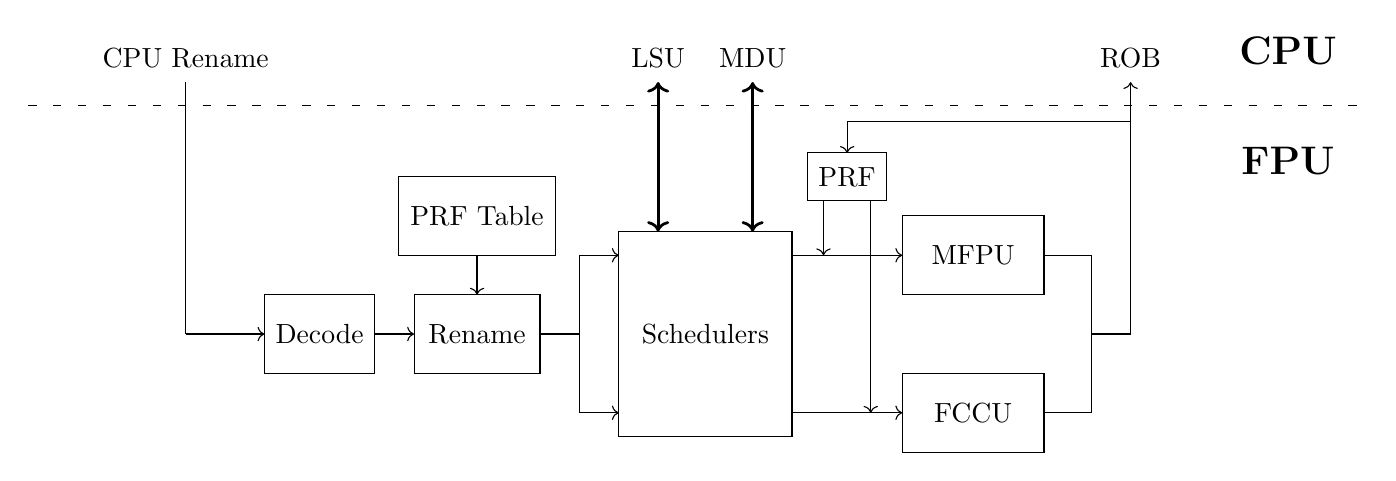
\begin{tikzpicture}
        %\draw [loosely dashed] (0,0)--(0,10); %较疏的线状虚线
        %\draw [loosely dashed] (5,0)--(5,10); %较疏的线状虚线
        %\draw [loosely dashed] (10,0)--(10,10); %较疏的线状虚线
        %\draw [loosely dashed] (20,0)--(20,10); %较疏的线状虚线
        %\draw (0,0) rectangle (15,7);

        \node at(1,6) {CPU Rename};
        \draw (1,5.7)--(1,2.5);
        \draw [->] (1,2.5)--(2,2.5);

        %decode
        \node at(2.7,2.5) {Decode};
        \draw (2,2) rectangle (3.4,3);

        \node at(4.7,2.5) {Rename};
        \draw (3.9,2) rectangle (5.5,3);
        \draw [->] (3.4,2.5)--(3.9,2.5);

        \node at(4.7,4) {PRF Table};
        \draw (3.7,3.5) rectangle (5.7,4.5);
        \draw [->] (4.7,3.5)--(4.7,3);

        \draw (5.5,2.5)--(6,2.5)--(6,3.5);
        \draw (6,2.5)--(6,1.5);
        \draw [->] (6,3.5)--(6.5,3.5);
        \draw [->] (6,1.5)--(6.5,1.5);
        \node at(7.6,2.5) {Schedulers};
        \draw (6.5,1.2) rectangle (8.7,3.8);

        \draw [<->, line width=1pt] (7,5.7)--(7,3.8);
        \draw [<->, line width=1pt] (8.2,5.7)--(8.2,3.8);
        \node at(7,6) {LSU};
        \node at(8.2,6) {MDU};

        \draw [->] (8.7,3.5)--(10.1,3.5);
        \draw [->] (8.7,1.5)--(10.1,1.5);
        \node at(9.4,4.5) {PRF};
        \draw (8.9,4.2) rectangle (9.9,4.8);
        \draw [->] (9.1,4.2)--(9.1,3.5);
        \draw [->] (9.7,4.2)--(9.7,1.5);

        \node at(11,3.5) {MFPU};
        \node at(11,1.5) {FCCU};
        \draw (10.1,1) rectangle (11.9,2);
        \draw (10.1,3) rectangle (11.9,4);

        \draw (11.9,1.5)--(12.5,1.5)--(12.5,2.5);
        \draw (11.9,3.5)--(12.5,3.5)--(12.5,2.5);
        \node at(13,6) {ROB};
        \draw (12.5,2.5)--(13,2.5);
        \draw [->] (13,2.5)--(13,5.7);
        \draw (13,5.2)--(9.4,5.2);
        \draw [->] (9.4,5.2)--(9.4,4.8);

        \draw [loosely dashed] (-1,5.4)--(16,5.4);
        \node at(15,6.1) {\Large{\textbf{CPU}}};
        \node at(15,4.7) {\Large\textbf{FPU}};
        
    \end{tikzpicture}
    \caption{FPU整体结构}
    \label{fig:enter-label}
\end{figure}

FPU部分没有自己的取指、访存和提交部件,这些是依赖于整数部分的。当指令通过整数部分的译码阶段后,若其需要在FPU部分被执行,或根本未被识别(整数部分的译码器仅对少数依赖整数部分的浮点指令进行译码,大部分浮点指令在FPU内译码),则在下一周期被发射到FPU中(此时其也在ROB中被分配表项,这是与整数部分共用的),FPU每周期仅接受一条指令。当浮点指令执行结束后,会将结果写回ROB,和其它指令一样被正常提交。

FPU在执行阶段具有两个功能单元,一个用于执行大部分浮点运算(称为MFPU),另一个用于执行涉及浮点条件码(FCC)的指令(称为FCCU),例如浮点比较、条件传送和条件分支。二者的保留站容量皆为4,MFPU的保留站是乱序发射的,这和ALU是完全一致的。FCCU的保留站是严格顺序发射的FIFO结构,这个思路和MDU一致,令FCCU持有FCC的临时版本,顺序通过FCCU的指令可直接修改或使用FCCU持有的FCC,并在提交时对FCC作出持久性修改,清空流水线时将FCCU持有的FCC重置为提交的版本。MFPU和FCCU各自负责执行的指令如表2.5所示。

\begin{table}[htb]
\centering
\caption{浮点指令所需功能单元分类}
    \label{fig:enter-label}
\begin{tabular}{m{3.5cm}<{\centering}|m{7cm}<{\centering}}
\hline  % 一条水平线
\textbf{功能单元类型} & \textbf{指令}\\
\hline
\textbf{MFPU} & abs.fmt, add.fmt, ceil.fmt, cvt.d.fmt, cvt.s.fmt, cvt.w.fmt, div.fmt, floor.w.fmt, ldc1, lwc1, mfc1, mov.fmt, movn.fmt, movz.fmt, mtc1, mul.fmt, neg.fmt, round.fmt, sdc1, sqrt.fmt, sub.fmt, swc1, trunc.fmt \\
\hline
\textbf{FCCU} & bc1f, bc1t, c.cond.fmt, movf, movf.fmt, movt, movt.fmt \\
\hline
\end{tabular}

\end{table}

\subsection{浮点寄存器(FPR)及其重命名}

MIPS32定义了FPR[0]-FPR[31]共32个32位的浮点寄存器,为提供双精度支持,FPR[2i]和FPR[2i+1]可映射为一个64位浮点寄存器使用,浮点指令的操作数即为32位或64位的浮点寄存器。因此,Ma-River的FPU对于浮点寄存器采取了奇偶分体的策略,源操作数和目的操作数都仅保留寄存器编号高4位,使用信号和写回信号都分为奇偶两组,这样简化了双精度浮点运算指令的“使用4个FPR,写回2个FPR”的复杂行为。

Ma-River CPU在FPU部分的寄存器重命名采取基于物理寄存器(PRF)的策略,这和整数部分使用ROB不同,并不对FPR设置真正的寄存器文件,其提交值和未提交值都在PRF中。PRF也是奇偶分体的,总共64个32位寄存器,奇FPR使用奇PRF,偶FPR使用偶PRF。我们记录每个PRF的状态及FPR对应的PRF,在FPU的寄存器重命名阶段为目的操作数分配一个空闲的PRF,并且查询源操作数的PRF编号。指令执行结束后将结果写到PRF中,发射时直接读取PRF值(由于PRF也保存提交后的值,此时一定是有效的),指令提交时,其写回的PRF值变为提交值,令目的操作数对应的上一个PRF空闲(此时不可能有使用它的指令了)。当流水线被清空时,未被提交的PRF将变为空闲状态。

\subsection{浮点控制寄存器(FCR)}

FCR对于FPU犹如CP0寄存器对于CPU,它们设置FPU的一般行为并反映FPU的状态。Ma-River CPU实现了MIPS32定义的全部5个FCR,如表2.6所示,可以通过cfc1/ctc1指令读写它们。

\begin{table}[htbp]
\centering
\caption{Ma-River CPU支持的FCR}
    \label{fig:enter-label}
\begin{tabular}{c|c}
\hline  % 一条水平线
\textbf{FCR} & \textbf{说明}\\
\hline
FIR & 描述FPU实现的特性\\
% \hline
FCSR & 描述FPU的条件和异常状态,设置舍入/规格化规则\\
% \hline
FCCR & 即浮点条件码FCC\\
% \hline
FEXR & 浮点异常位\\
% \hline
FENR & 异常屏蔽位,设置舍入/规格化规则\\
\hline

\end{tabular}

\end{table}

\subsection{浮点异常}

MIPS32(IEEE754)针对浮点运算中的一些特殊情况定义了如下所示的6种浮点异常,它们都对应于CPU的FPE异常,发生FPE时由FCSR.Cause指示异常原因。部分浮点异常是可屏蔽的,若被屏蔽则将结果置为特殊值(0、$\infty$、NaN)。Ma-River CPU正确实现了它们。

\begin{itemize}
    \item \textbf{未实现的运算} \quad 由于Ma-River实现了MIPS32 Release1定义的所有单/双精度和定点数运算,在指令被识别的情况下不会引发此异常。未被识别的指令引发保留指令异常。
    \item \textbf{非法运算} \quad 运算操作数中有NaN,或者执行了$\frac 0 0$、$\frac{\infty}{\infty}$、对负数开根这样的结果未定义操作。若其被屏蔽则结果置为NaN。
    \item \textbf{除0} \quad 当除法运算的分子非0且分母为0。若其被屏蔽则结果置为$\infty$。
    \item \textbf{上溢} \quad 结果绝对值超出单/双精度的最大表示范围,若其被屏蔽则结果置为$\infty$。
    \item \textbf{下溢} \quad 当结果为非0非规格化数时。若其被屏蔽则按舍入规则处理。
    \item \textbf{结果不精确} \quad 产生上溢或下溢时,或舍入导致结果不精确。若其被屏蔽则按舍入规则处理。
\end{itemize}

除了标准的浮点异常以外,Ma-River CPU的FPU还可能会引发保留指令异常(在FPU被实现的情况下,保留指令是FPU的译码阶段负责检测的)和协处理器不可用异常(Status.CU1置0但执行了浮点指令,一般是操作系统未为当前线程启用FPU)。无论引发哪种异常,FPU都会写回ROB,在提交时按照CPU异常机制正常处理。

\subsection{FPU与CPU的数据交互}

FPU的访存指令需要使用整数部分的访存单元,此外还有一些指令具有在FPR和GPR间传送数据或者同时使用GPR和FPR的行为,无论如何,它们需要在整数部分的译码阶段就被识别,并且在此之后既需要发射到FPU,又需要继续在整数部分的流水线中执行,即一条指令拆为两个微指令执行,这两个微指令(根据同一个ROB编号确定)需要在两个部分中“内外接应”,实现数据的交互。我们据此把浮点指令作出了如下分类:

\begin{itemize}
    \item \textbf{不需FPR}(cfc1, ctc1)\quad 它们只读写CP1控制寄存器,作为正常CPU指令执行即可,处理方式同mfc0/mtc0。
    \item \textbf{需要单个FPR值(或FCC),写回GPR}(movf, movt, mfc1) \quad 我们将这些指令的整数部分微指令安排在MDU中执行,在整数部分设置一个以ROB编号寻址的Buffer,MDU保留站中需要FPR值的指令要等到Buffer对应位置有效才可发射。当MFPU/FCCU保留站的微指令被发射时,此时必然得到FPR操作数值(或者在FCCU执行指令时得到FCC值),将其通过通道传送到整数部分的Buffer中并尝试唤醒MDU保留站中的指令。这样,MDU保留站发射指令时即可得到所需的FPR值,无论两个微指令在两条流水线中相对位置是什么样的。
    \item \textbf{需要单个GPR值,写回FPR}(movn.fmt, movz.fmt, mtc1)\quad 和上述情形相反,我们同样地设置一个MDU保留站到MFPU的数据通道与Buffer即可。
    \item \textbf{FPR访存}(ldc1, lwc1, sdc1, swc1)\quad 和上述情形类似,只不过换成了Mem保留站以及LSU的写回ROB阶段与MFPU的双向数据传输,需要设置相应的Buffer。此外,ldc1和sdc1是64位的访存指令,我们可在Mem保留站发射它们时将其进一步拆为两个连续发射的32位访存微指令。
    \item \textbf{仅使用FPR} \quad 剩余所有浮点指令,无需和整数部分交互。
\end{itemize}

\subsection{浮点运算及其执行部件}

表2.7列出了MIPS32定义的主要的浮点运算类型及Ma-River中的执行延迟(从发射到写回ROB的周期数),Ma-River CPU正确地实现了它们,使用我们自行实现的运算部件(主要使用MFPU,仅有浮点比较在FCCU中实现),无需额外IP核。由于浮点运算较为复杂,为避免影响CPU频率,我们采取了较为保守的长流水线设计,流水段拆分较细,执行延迟略高。

\begin{table}[htbp]
\centering
\caption{Ma-River CPU实现的浮点运算类型}
    \label{fig:enter-label}
\begin{tabular}{c|c|c}
\hline  % 一条水平线
\textbf{浮点运算类型} & \textbf{指令} & \textbf{执行延迟}\\
\hline
加减 & add.fmt, sub.fmt & 12\\
% \hline
变号 & abs.fmt, neg.fmt & 1\\
% \hline
乘法 & mul.fmt & 13\\
% \hline
除法 & div.fmt & 60\\
% \hline
平方根 & sqrt.fmt & 60\\
% \hline
比较 & c.cond.fmt & 3\\
% \hline
转换为浮点(精度转换) & cvt.s, cvt.d & 10\\
% \hline
转换为定点(取整) & cvt.w, ceil.fmt, floor.fmt, round.fmt, trunc.fmt & 6\\
\hline
\end{tabular}

\end{table}

负责执行大部分运算的MFPU结构如图3所示。MFPU采用单入单出的动态多功能流水线结构,除了除法和开根以外,所有运算部件都是完全流水化的,不同类型运算可重叠执行,但共用一部分流水线(例如舍入和规格化),这节省了部件。共用输出端的不同部件若同时输出,需按照复杂运算优先的原则进行仲裁,阻塞其它部件。

\begin{figure}[htbp]
    \centering
    \begin{tikzpicture}

        \node at(0,6.4) {\Large Input};
        \draw [->] (0,6)--(1.3,6);
        \node at(2.1,6) {Prepare};
        \draw (1.3,5.5) rectangle (2.9,6.5);

        \draw (2.9,6)--(3.5,6);
        \draw (3.5,10.8)--(3.5,1.2);
        \draw [->] (3.5,10.8)--(4,10.8);
        \draw [->] (3.5,9.2)--(4,9.2);
        \draw [->] (3.5,7.6)--(4,7.6);
        \draw [->] (3.5,6)--(4,6);
        \draw [->] (3.5,4.4)--(4,4.4);
        \draw [->] (3.5,2.8)--(4,2.8);

        \node at(5,2.8) {ToFixed};
        \node at(5,4.4) {ToFloat};
        \node at(5,6) {Sqrt};
        \node at(5,7.6) {Div};
        \node at(5,9.2) {Mul};
        \node at(5,10.8) {Add};
        \draw (4,2.3) rectangle (6,3.3);
        \draw (4,3.9) rectangle (6,4.9);
        \draw (4,5.5) rectangle (6,6.5);
        \draw (4,7.1) rectangle (6,8.1);
        \draw (4,8.7) rectangle (6,9.7);
        \draw (4,10.3) rectangle (6,11.3);

        \draw (6,10.8)--(6.5,10.8);
        \draw (6,9.2)--(6.5,9.2);
        \draw (6,7.6)--(6.5,7.6);
        \draw (6,6)--(6.5,6);
        \draw (6,4.4)--(6.5,4.4);
        \draw (6.5,10.8)--(6.5,4.4);
        \draw [->] (6.5,7.6)--(7,7.6);

        \node at(7.9,7.6) {Nomalize};
        \draw (7,7.1) rectangle (8.8,8.1);
        \draw [->] (8.8,7.6)--(9.3,7.6);

        \node at(10.1,7.6) {Round};
        \draw (9.3,7.1) rectangle (10.9,8.1);
        \draw (10.9,7.6)--(11.4,7.6);
        \draw (6,2.8)--(11.4,2.8);
        \draw (3.5,1.2)--(11.4,1.2)--(11.4,7.6);
        \draw [->] (11.4,6)--(12.7,6);
        \node at(12.7,6.4) {\Large Result};
        
    \end{tikzpicture}
    \caption{MFPU结构}
    \label{fig:enter-label}
\end{figure}

\begin{itemize}
    \item \textbf{准备阶段} \quad 对于单/双精度浮点类型的操作数,将其统一按双精度处理(这样无需再设计不同精度的运算部件),提取指数和尾数,判断0、无穷和NaN。对于一些简单的变号(abs、neg)或传送指令,在此阶段后可直接输出结果。
    \item \textbf{加法} \quad 浮点加法器有3个流水段,第一个流水段进行指数减法,第二个流水段进行尾数对齐,第三个流水段进行尾数加法。
    \item \textbf{乘法} \quad 浮点乘法器有4个流水段,同时进行53位的尾数乘法和指数加法,尾数乘法同样可通过配置选项选用基于LUT的Wallace Tree或基于DSP的分段乘法,由于53位乘法的Wallace Tree消耗巨量的LUT,我们最终的提交版本是选用DSP的。
    \item \textbf{除法} \quad 浮点除法器是非流水的,尾数使用朴素的53位移位除法。
    \item \textbf{平方根} \quad 浮点平方根使用快速移位算法对尾数(需将指数调整为偶数再除2)进行开根,过程和时间开销类似于除法。
    \item \textbf{定点转浮点} \quad 定点数(整数)到浮点数转换有2个流水段,第一个流水段计算指数,第二个流水段移位得到尾数。
    \item \textbf{浮点转定点} \quad 浮点数到定点数转换有3个流水段,第一个流水段进行尾数移位,第二个流水段进行舍入,第三个流水段进行取负和无效值检测。
    \item \textbf{规格化阶段} \quad 规格化部件接受上述生成浮点数结果运算部件产生的符号、指数和108位尾数(此时还是中间状态),将尾数移位为1.xxx的规格化形式(即便结果实际上是非规格化数)。这一阶段有3个流水段,前2个流水段计算尾数前导0个数,第三个流水段对尾数进行移位。
    \item \textbf{舍入阶段} \quad 舍入部件根据FCSR.RM指示的舍入规则,生成真正的单/双精度结果。这一阶段有3个流水段,第一个流水段计算真正的指数值,第二个流水段进行尾数舍入,第三个流水段进行结果调整并判断上下溢。
\end{itemize}

\section{外部接口}

Ma-River CPU核对外仅通过一个用于访存的AXI3总线接口和6根高电平有效的中断相连。

取指部件和访存部件都具有自己的AXI接口,二者在内部通过一个简单的仲裁器合并为一条对外连接的总线。

\section{性能}

在大赛的性能测试中,Ma-River CPU的频率最高可达118MHz。在我们最终运行Linux的SoC上,我们将CPU和SoC频率皆设置为100MHz。

Ma-River CPU在大赛性能测试10个benchmark的表现如表2.8所示,相对GS132的平均加速比高达110.50,平均IPC比为46.71,平均IPC为1.32。

\begin{table}[htbp]
\centering
\caption{性能测试表现}
\label{fig:enter-label}
\begin{tabular}{c|c|c|c}
\hline  % 一条水平线
\textbf{测试程序} & \textbf{加速比} & \textbf{IPC} & \textbf{IPC比值}\\
\hline
bitcount & 112.54 & 1.45 & 47.06 \\
% \hline
bubble\_sort & 119.29 & 1.31 & 50.47\\
% \hline
coremark & 85.00 & 1.04 & 35.96\\
% \hline
crc32 & 132.02 & 1.62 & 55.87\\
% \hline
dhrystone & 106.71 & 1.29 & 45.15\\
% \hline
quick\_sort & 83.45 & 1.01 & 35.31\\
% \hline
select\_sort & 118.81 & 1.53 & 50.27\\
% \hline
sha & 133.29 & 1.60 & 56.40\\
% \hline
streamcopy & 116.60 & 1.24 & 49.42\\
% \hline
stringsearch & 109.58 & 1.25 & 46.37\\
% \hline
几何平均 & 110.50 & 1.32 & 46.71\\
\hline
\end{tabular}

\end{table}

此外,我们还在Linux环境下(CPU和SoC频率均为100MHz)对Ma-River CPU的浮点性能进行了测试,Linpack测试结果为3.23MFLOPS。
% Part 3 SoC设计


\chapter{SoC与外设}

\section{概述}

我们致力于构建一套能提供\textbf{真正PC机体验}的SoC与外设系统。目前我们已驱动VGA、LCD、PS/2、GPIO、触摸、DDR、串口、以太网等一系列外设,初步达成了这一目标。其中,VGA、LCD、PS/2、GPIO的控制器和对应驱动为团队自行实现。

实机效果如图3.1所示。

%开始插入图片
\begin{figure}[htb] % htbp代表图片插入位置的设置
\centering %图片居中
%添加图片;[]中为可选参数,可以设置图片的宽高;{}中为图片的相对位置
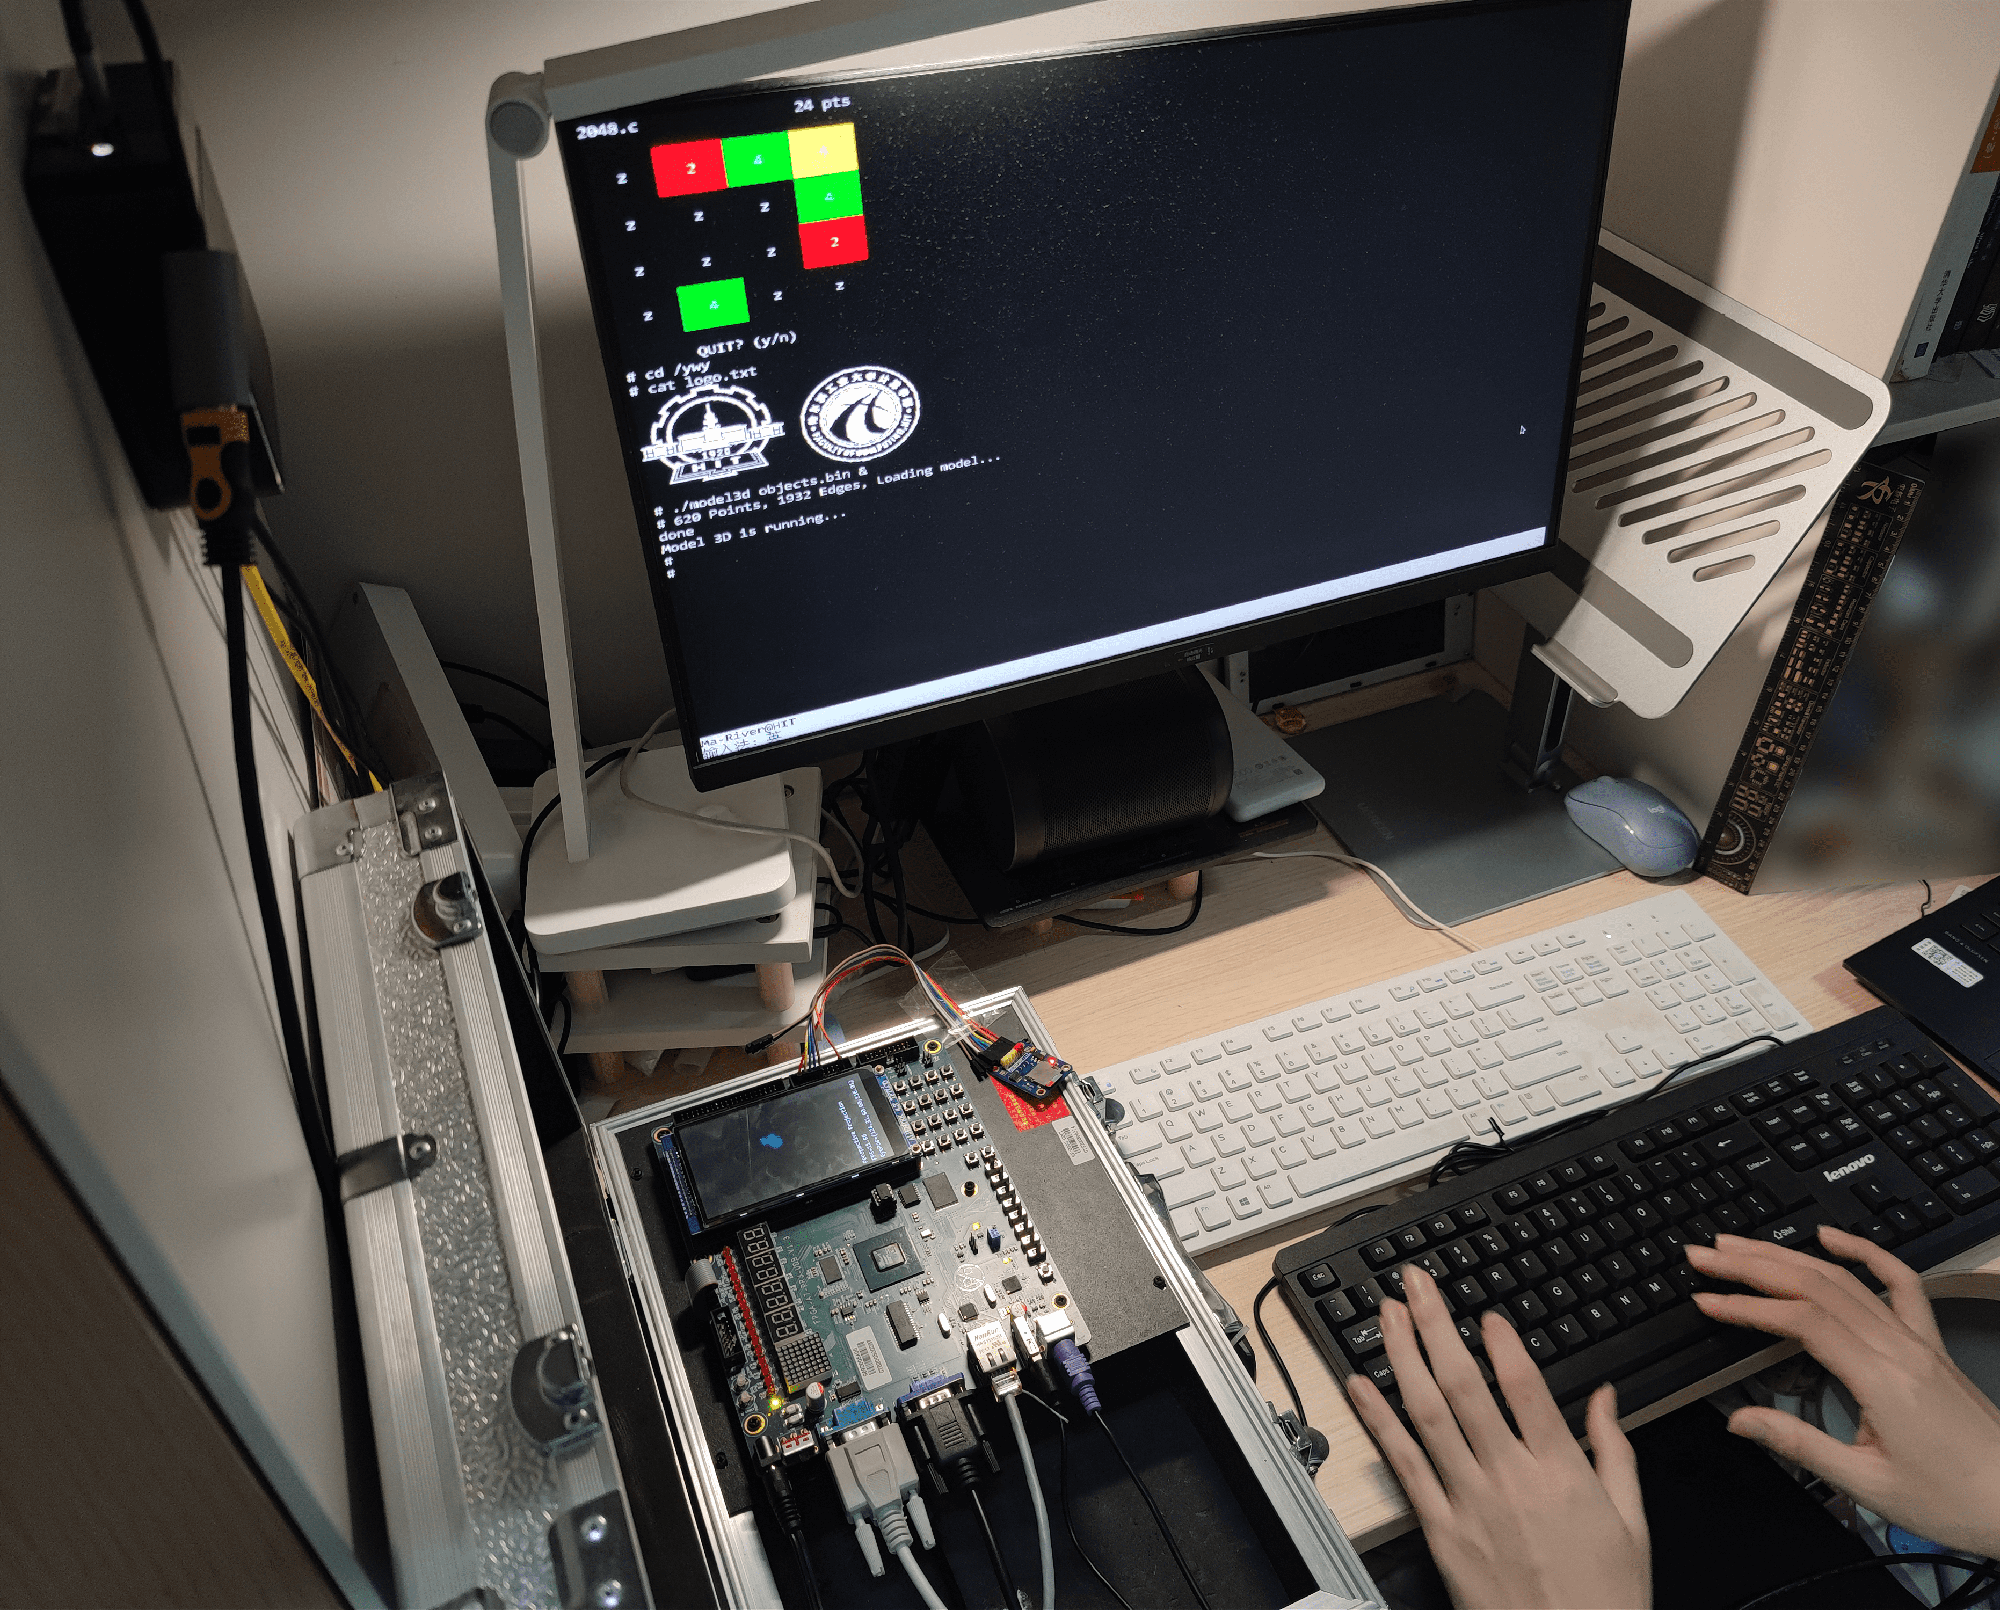
\includegraphics[width=12cm]{img/sys.png}
\caption{实机效果展示} % 图片标题
\label{pic1} % 图片标签
\end{figure}

\newpage

\section{整体架构}

SoC整体架构如下图所示:

\begin{figure}[!ht]
    \centering
    \begin{tikzpicture}[myrect/.style={rounded corners,draw=vivadodraw,fill=vivadofill}]
    
    
    \draw[myrect] (0,0) rectangle (235pt,30pt);
    \node[centered=0,font=\fontsize{9}{9}\selectfont,node font=\sffamily] (VGA) at (117.5pt, 15pt) {DDR};
    % 左半部分
    \draw[myrect] (0,45pt) rectangle (75pt,75pt);
    \draw[myrect] (0,90pt) rectangle (75pt,120pt);
    \draw[myrect] (0,135pt) rectangle (75pt,165pt);
    \draw[myrect] (0,180pt) rectangle (75pt,210pt);
    \draw[myrect] (0,225pt) rectangle (75pt,255pt);
    
    \node[centered=0,font=\fontsize{9}{9}\selectfont,node font=\sffamily] (VGA) at (37.5pt, 60pt) {VGA Controller};
    \node[above=45pt,centered=0,font=\fontsize{9}{9}\selectfont,node font=\sffamily] (USB) at (VGA) {USB Host Ctl};
    \node[above=45pt,centered=0,font=\fontsize{9}{9}\selectfont,node font=\sffamily] (IIC) at (USB) {AXI IIC};
    \node[above=45pt,centered=0,font=\fontsize{9}{9}\selectfont,node font=\sffamily] (Eth) at (IIC) {AXI EthernetLite};
    \node[above=45pt,centered=0,font=\fontsize{9}{9}\selectfont,node font=\sffamily] (INTC) at (Eth) {AXI INTC};
    
    % 中间
    \draw[myrect] (90pt,45pt) rectangle (145pt,255pt);
    \node[centered=0,font=\fontsize{9}{9}\selectfont,node font=\sffamily,align=center] at (117.5pt,150pt) {AXI \\
                   Interconnect};
    
    % 右半部分
    \draw[myrect] (160pt,45pt) rectangle (235pt,75pt);
    \draw[myrect] (160pt,90pt) rectangle (235pt,120pt);
    \draw[myrect] (160pt,135pt) rectangle (235pt,165pt);
    \draw[myrect] (160pt,180pt) rectangle (235pt,210pt);
    \draw[myrect] (160pt,225pt) rectangle (235pt,255pt);
    
    \node[centered=0,font=\fontsize{9}{9}\selectfont,node font=\sffamily] (LCD) at (197.5pt, 60pt) {LCD Controller};
    \node[above=45pt,centered=0,font=\fontsize{8.5}{8.5}\selectfont,node font=\sffamily] (BRAM) at (LCD) {Bootloader BRAM};
    \node[above=45pt,centered=0,font=\fontsize{9}{9}\selectfont,node font=\sffamily] (PS2) at (BRAM) {PS/2};
    \node[above=45pt,centered=0,font=\fontsize{9}{9}\selectfont,node font=\sffamily] (UART) at (PS2) {AXI UART};
    \node[above=45pt,centered=0,font=\fontsize{9}{9}\selectfont,node font=\sffamily] (GPIO) at (UART) {GPIO\&Clock};
    
    % 顶部
    \draw[myrect] (0pt,270pt) rectangle (235pt,300pt);
    \node[centered=0,font=\fontsize{9}{9}\selectfont,node font=\sffamily] (VGA) at (117.5pt, 285pt) {CPU};
    
    
    % AXI Master
    \draw[very thick,->] (117.5pt, 270pt) -- (117.5pt, 255pt); % CPU
    \draw[very thick,->] (37.5pt, 45pt) -- (37.5pt, 30pt); % VGA DMA
    \draw[very thick,->] (197.5pt, 45pt) -- (197.5pt, 30pt); % LCD DMA
    
    % AXI Slave
    \draw[thick,->] (90pt, 60pt) -- (75pt, 60pt);
    \draw[thick,->] (90pt, 105pt) -- (75pt, 105pt);
    \draw[thick,->] (90pt, 150pt) -- (75pt, 150pt);
    \draw[thick,->] (90pt, 195pt) -- (75pt, 195pt);
    \draw[thick,->] (90pt, 240pt) -- (75pt, 240pt);
    
    \draw[thick,->] (145pt, 60pt) -- (160pt, 60pt);
    \draw[thick,->] (145pt, 105pt) -- (160pt, 105pt);
    \draw[thick,->] (145pt, 150pt) -- (160pt, 150pt);
    \draw[thick,->] (145pt, 195pt) -- (160pt, 195pt);
    \draw[thick,->] (145pt, 240pt) -- (160pt, 240pt);
    
    \draw[thick,->] (117.5pt, 45pt) -- (117.5pt, 30pt);
    
    % Interrupts
    \draw[dashed,-latex] (0pt, 105pt) -- (-15pt, 105pt) -- (-15pt, 242pt) -- (0pt,242pt); % USB
    \draw[dashed,-latex] (0pt, 150pt) -- (-10pt, 150pt) -- (-10pt, 237pt) -- (0pt,237pt); % IIC
    \draw[dashed,-latex] (0pt, 195pt) -- (-5pt, 195pt) -- (-5pt, 231pt) -- (0pt,231pt); % Eth
    
    \draw[dashed,-latex] (235pt, 60pt) -- (255pt, 60pt) -- (255pt, 294pt) -- (235pt,294pt); % LCD
    \draw[dashed,-latex] (235pt, 150pt) -- (250pt, 150pt) -- (250pt, 288pt) -- (235pt,288pt); % PS/2
    \draw[dashed,-latex] (235pt, 195pt) -- (245pt, 195pt) -- (245pt, 282pt) -- (235pt,282pt); % UART
    \draw[dashed,-latex] (235pt, 240pt) -- (240pt, 240pt) -- (240pt, 276pt) -- (235pt,276pt); % GPIO
    
    \draw[dashed,-latex] (0pt, 248pt) -- (-15pt, 248pt) -- (-15pt, 285pt) -- (0pt,285pt); % INTC
    
    % 图注
    \draw[thick,->] (55pt, -10pt) -- (70pt, -10pt) node[right] {AXI总线};
    \draw[dashed,-latex] (140pt, -10pt) -- (155pt, -10pt) node[right] {中断};
    
    \end{tikzpicture}

    \caption{SoC整体架构} % 图片标题
    \label{pic_soc_all} % 图片标签
\end{figure}



\section{资源分配}

\subsection{外设地址}

\begin{table}[!ht]
\centering
\caption{设备物理地址分配}
\label{tab:pehi_addr}
\begin{tabular}{cc|cc}
\hline
设备名称           & 起始地址         & 设备名称                 & 起始地址                 \\ \hline
DDR3           & 0x0000\_0000 & VGA控制器               & 0x1FE0\_0000         \\
AXI IIC(触摸)    & 0x1FA0\_0000 & AXI UART16550        & 0x1FE4\_0000         \\
AXI INTC       & 0x1FB0\_0000 & AXI QUAD SPI     & 0x1FE8\_0000         \\
Bootloader ROM & 0x1FC0\_0000 & AXI Ethernetlite  &  0x1FF0\_0000                 \\
LCD控制器         & 0x1FD0\_0000 & \multicolumn{1}{l}{} & \multicolumn{1}{l}{} \\ \hline
\end{tabular}
\end{table}

\subsection{外设中断}

《MIPS指令系统规范》\footnote{参见龙芯杯2023发布包文档:《A03“系统能力培养大赛”MIPS指令系统规范v1.01》}中要求实现6个硬件中断,但计时器中断会复用 HW5 硬件中断,故可以直接使用的硬件中断只有5个,且仅支持电平触发中断;为了拓展中断数量、处理部分边沿触发的中断,我们使用了Xilinx AXI INTC IP核。

中断的连接关系如下图所示,其中AXI Ethernetlite为边沿触发中断,其他均为电平触发中断。

% Define color
\definecolor{vivadodraw}{rgb}{0.2549,0.3804,0.6235}
\definecolor{vivadofill}{rgb}{0.9294,0.9647,0.9960}


\begin{figure}[!ht]
    \centering
    
    \begin{tikzpicture}[myint/.style={anchor=east,inner sep=0,font=\fontsize{10}{10}\selectfont},node font=\sffamily]
    
    \draw[rounded corners,draw=vivadodraw,fill=vivadofill] (0, 0) rectangle (45pt, 140pt);
    
    \node[anchor=north] at (22.5pt, 0pt) {CPU INT};
    
    \node[myint] at (42pt, 120pt) {HW0};
    \node[myint] at (42pt, 100pt) {HW1};
    \node[myint] at (42pt, 80pt) {HW2};
    \node[myint] at (42pt, 60pt) {HW3};
    \node[myint] at (42pt, 40pt) {HW4};
    \node[myint] at (42pt, 20pt) {HW5};
    
    % \draw (45pt, 20pt) -- (55pt, 20pt) node[right] {保留};
    \draw (45pt, 100pt) -- (55pt, 100pt) node[right] {UART};
    \draw (45pt, 80pt) -- (55pt, 80pt) node[right] {GPIO\&Clock};
    \draw (45pt, 60pt) -- (55pt, 60pt) node[right] {LCD};
    \draw (45pt, 40pt) -- (55pt, 40pt) node[right] {PS/2};
    \draw (45pt, 20pt) -- (55pt, 20pt) node[right] {保留};
    
    
    \draw[->] (45pt, 120pt) -- (120pt, 120pt) -- (120pt, 100pt) -- (130pt, 100pt);
    
    \draw[rounded corners,draw=vivadodraw,fill=vivadofill] (130pt, 40pt) rectangle (175pt, 120pt);
    
    \node[anchor=north] at (152.5pt, 40pt) {AXI INTC};
    
    \node[myint] at (173pt, 100pt) {INTR0};
    \node[myint] at (173pt, 80pt) {INTR1};
    \node[myint] at (173pt, 60pt) {INTR2};
    
    \draw[blue,thick] (175pt, 100pt) -- (185pt, 100pt) node[right] {AXI Ethernetlite};
    \draw (175pt, 80pt) -- (185pt, 80pt) node[right] {AXI IIC};
    \draw (175pt, 60pt) -- (185pt, 60pt) node[right] {AXI QUAD SPI};
    
    \end{tikzpicture}

    \caption{中断的连接关系} % 图片标题
    \label{pic_intr} % 图片标签
\end{figure}



\section{外设说明}

\subsection{VGA}

实验板提供了标准VGA接口,我们为此自行设计并实现了具有文本和图像两种工作模式的VGA控制器,其分辨率和刷新率固定为1024×768@60Hz,位深度为4,能实现文本或图像的输出。

在文本模式下,VGA控制器按照8×16大小为一个格子,将屏幕划分为48行128列,每个格子可显示一个单色ASCII字符或半个汉字(两个格子显示一个汉字)。VGA控制器为ASCII字符内置了点阵字库,只需要通过AXI总线向对应地址写入颜色信息和字符的ASCII码即可显示对应的字符。为支持汉字等高级字符集,文本模式支持向格子中写入基于位的二值化图像信息(每个像素用一个位表示),只要在软件字库中添加自定义的点阵信息,即可显示任何语言的字符。此外,文本模式还具有可配置的闪烁光标。文本模式的全部图像信息直接使用片上BRAM存储,不需要消耗内存带宽,性能友好。

在图像模式下,无法直接在片上存储的图像数据只能通过DMA方式传输。VGA控制器会周期性地通过AXI总线从DDR中读取指定地址处的图像数据,显存地址和图像的显示区域由软件动态设置。基于图像模式和DMA机制,我们实现并移植了FrameBuffer驱动,能够实现虚拟终端、动画绘制、GUI应用等。

我们为U-Boot、ucore和Linux都移植了基于VGA控制器文本模式的Console驱动程序,使得用户可以直接使用VGA与系统进行交互。

\subsection{LCD及触摸}

实验板提供了分辨率为480*800的LCD屏幕,我们为其自行设计实现了LCD控制器实现文本与图像输出。LCD控制器也具有文本模式和图像模式。

LCD控制器的文本模式和VGA类似,故不再赘述。原则上系统Console也可使用LCD文本模式输出,但由于LCD屏幕太小,我们最终并未实现。

由于LCD本身具有显存,LCD的图像模式支持直接向屏幕某位置写入像素值,这会在单个像素上花费较多周期,CPU需要进行多次高代价uncached访存。为加速LCD图像绘制,我们也为LCD提供了DMA传输支持。软件可将像素数据准备在DDR中,设置LCD控制器的传输地址和范围即可启动单次DMA传输,LCD控制器会连续向显存中写入像素,传输完成后通过中断告知CPU。这使得我们基于LCD的动画应用可以以至少20~30FPS的帧率播放。基于其DMA机制,我们也实现并移植了和VGA类似的标准FrameBuffer驱动。

对于LCD的触摸功能,我们使用Xilinx AXI IIC IP核与LCD上的GT1151Q触摸芯片进行I2C通信,定时查询触摸状态,读取触摸坐标。

\subsection{PS/2键盘}

实验板提供了PS/2物理接口,我们为此自行设计并实现了简单的PS/2键盘控制器。它能够解析输入的PS/2物理信号,在按键按下或松开时发起键盘中断,读取来自键盘的扫描码。我们为键盘分配了单独的中断信号并将其连接到CPU的外部中断信号上,CPU可以通过AXI总线读取扫描码并响应中断。同时,我们使用了深度为4的FIFO对多个未读取的键盘扫描码进行缓冲。此外,对于不使用中断方式输入的系统(如U-Boot),可使用轮询方式读取扫描码。	

我们为PS/2键盘控制器编写了适配的驱动,结合VGA能达到实际PC机的体验。

\subsection{GPIO}
实验板上提供了LED、数码管、拨码开关、按键等GPIO设备,我们为此自行设计并实现了GPIO控制器以对它们进行读写以及可编程的中断控制。

\subsection{串口}
实验板提供了RS-232串行通信接口,我们使用官方提供的Xilinx UART16550进行驱动。该控制器的中断信号为电平触发,我们将其直接连接到CPU的外部中断信号上。

U-Boot和Linux源码中提供了相关驱动,可以直接使用。

\subsection{以太网}
实验板提供了以太网标准协议中的MDIO和MII接口。我们使用官方提供的Xilinx EthernetLite进行驱动。由于该IP仅提供上升沿触发的中断,我们使用中断控制器来转换中断类型。

U-Boot和Linux源码中提供了相关驱动,可以直接使用。

\subsection{SD卡}
我们通过实验板提供的拓展GPIO,连接了提供SPI接口的SD卡模块,故我们使用AXI QUAD SPI进行交互。

Linux源码中提供了相关驱动,可以直接使用。
% Part 4 系统软件
\chapter{系统软件}

\section{U-boot}

\subsection{背景}
U-Boot 是一个启动引导程序,常见于嵌入式系统中,用于引导 Linux 等操作系统。在本系统的设计中,U-Boot 将作为引导程序,放置在BRAM中;同时,我们根据展示需求,修改了U-boot源码以增加更多功能。

\subsection{移植内容}

\begin{itemize}
    \item 使用 U-boot v2023.07稳定版本
    \item 修改底层驱动,使其支持VGA Console+PS/2键盘输入输出
    \item 添加如图4.1所示的菜单启动界面,能够自动通过网口加载并选择性启动 Linux 或 ucore 操作系统
\end{itemize}

%开始插入图片
\begin{figure}[htb] % htbp代表图片插入位置的设置
\centering %图片居中
%添加图片;[]中为可选参数,可以设置图片的宽高;{}中为图片的相对位置
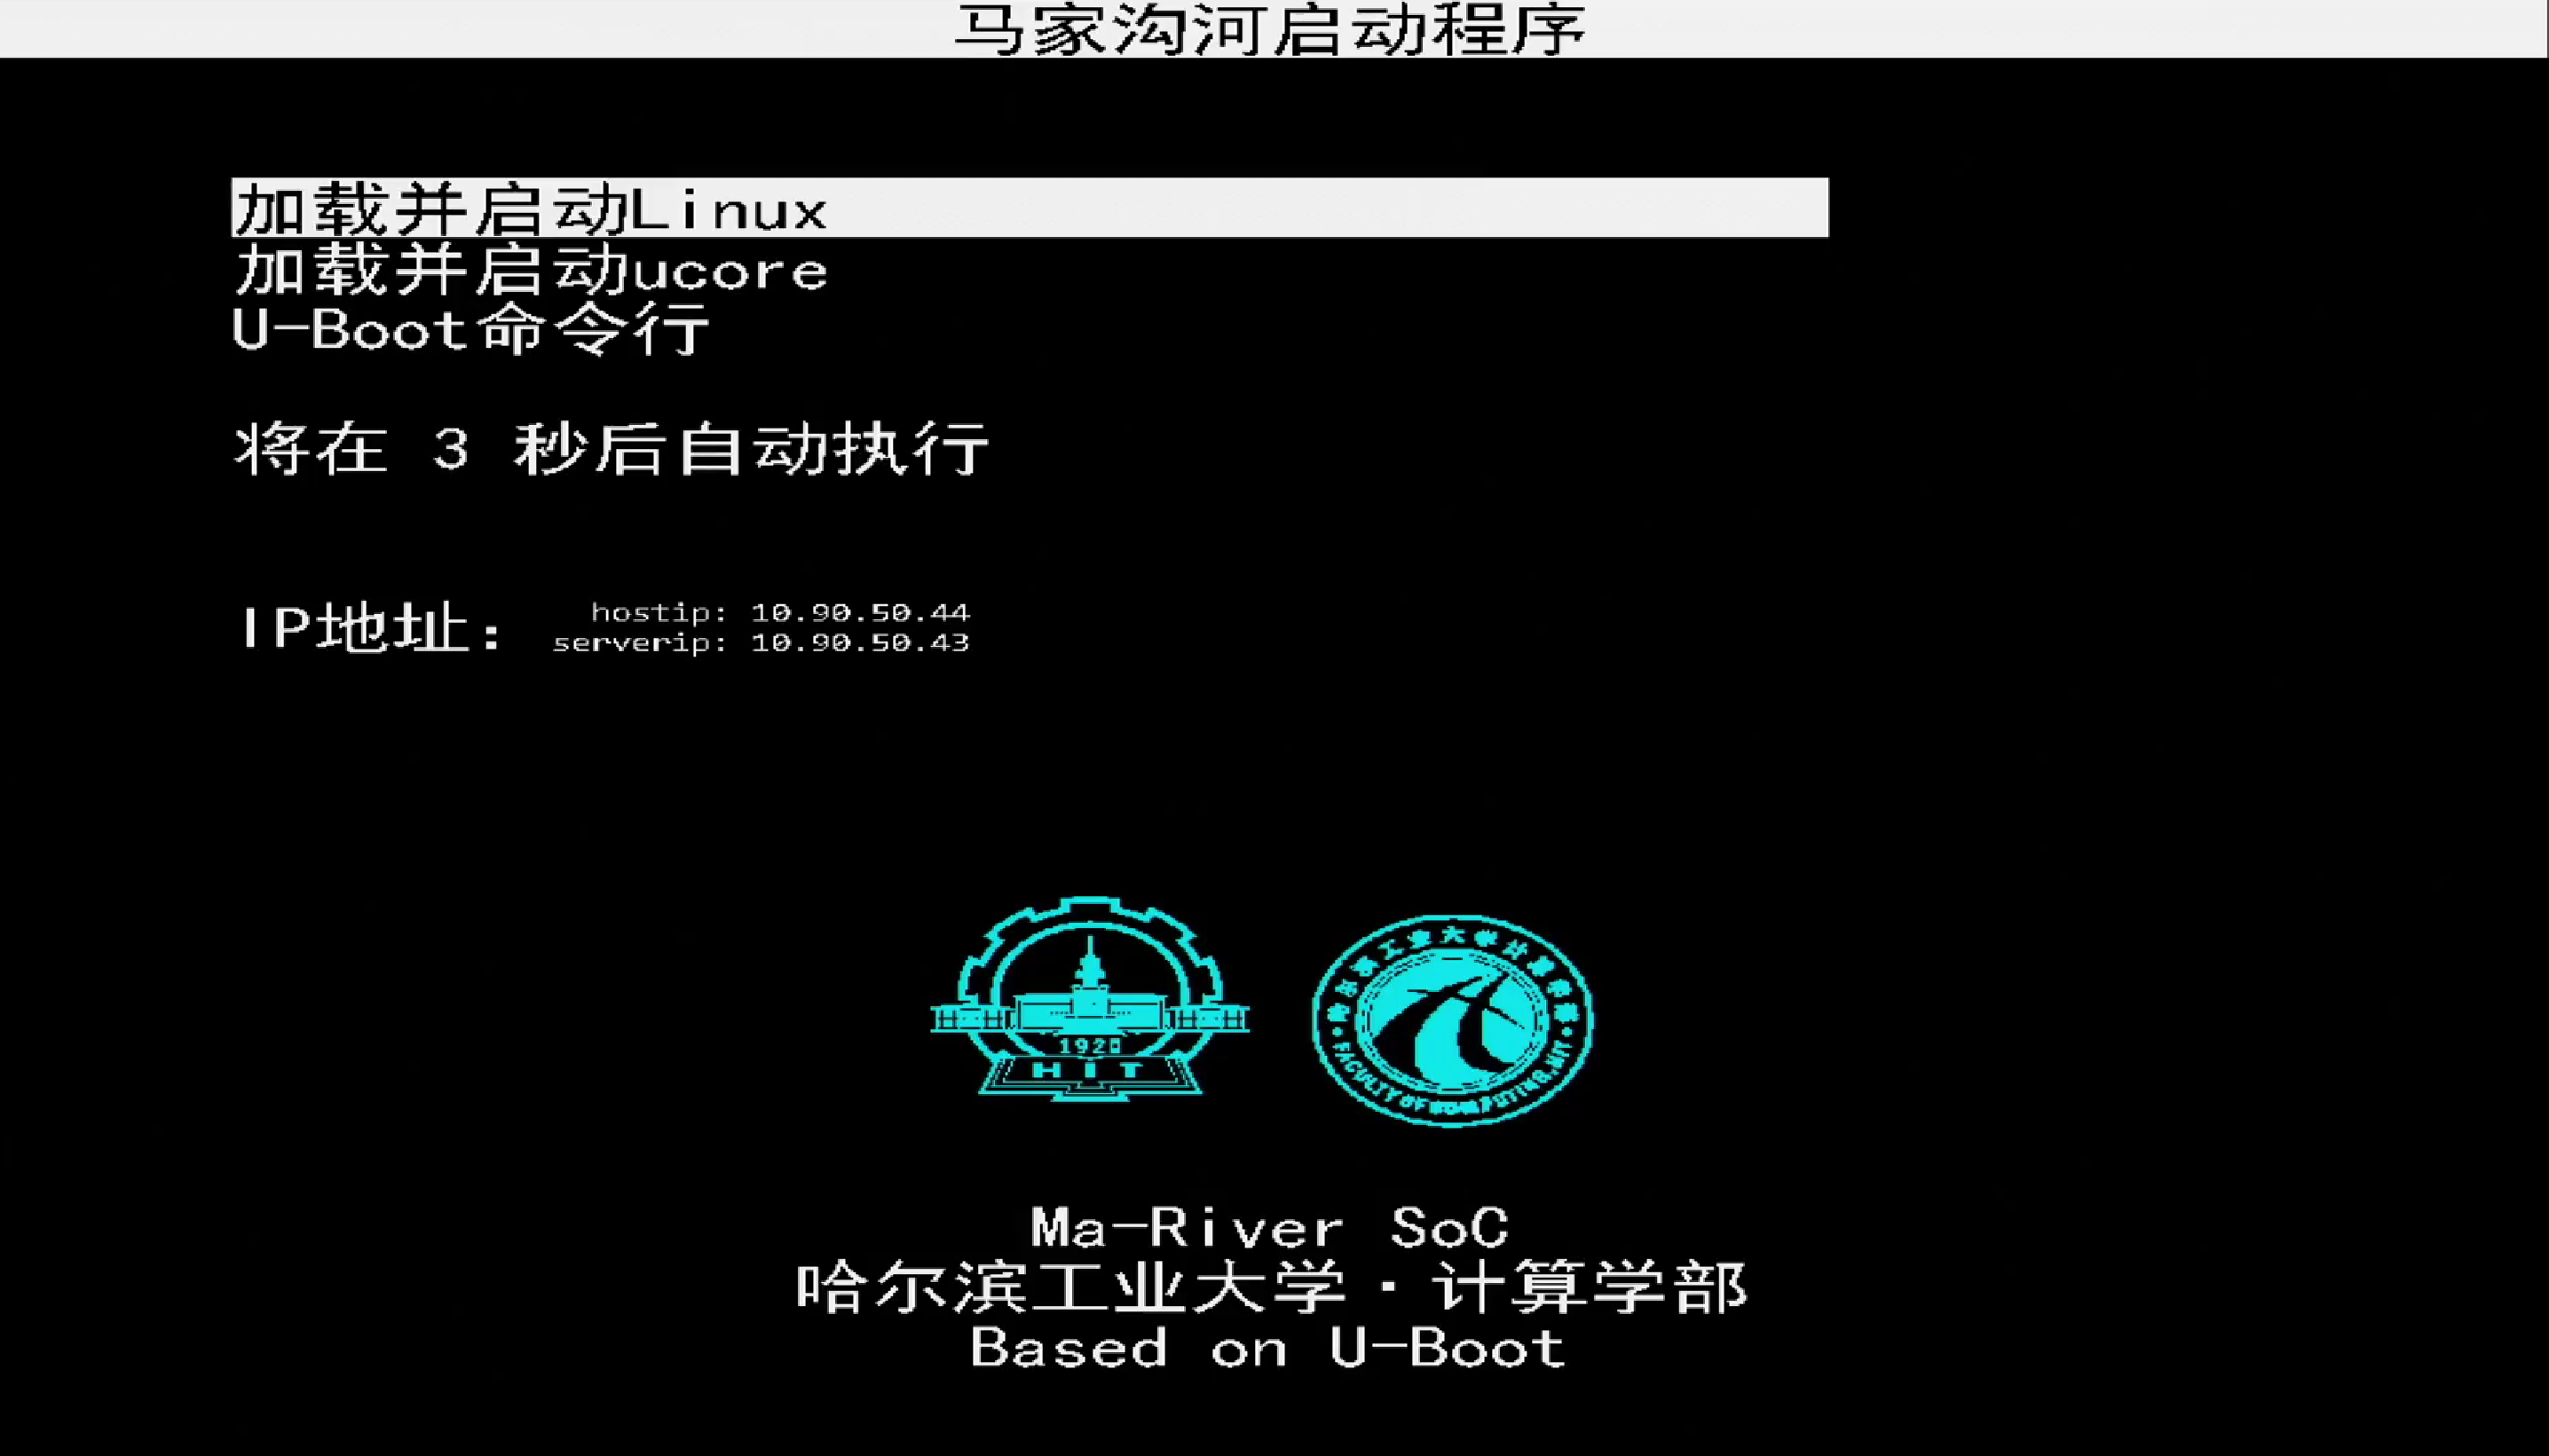
\includegraphics[width=13cm]{img/uboot.png}
\caption{U-Boot菜单启动界面} % 图片标题
\label{pic2} % 图片标签
\end{figure}

\section{ucore}

\subsection{背景}
ucore是清华大学的轻量级教学操作系统。

\subsection{移植内容}
\begin{itemize}
    \item 修改底层驱动,使其支持VGA Console+PS/2键盘输入输出
    \item 在U-Boot启动菜单中增加ucore自启动选项。
\end{itemize}

\section{Linux}
\subsection{背景}
Linux 是最为著名的开源操作系统,有丰富的软硬件支持。我们以最新的稳定版本 Linux v6.4 (2023年6月26日发布)作为基线进行移植。

\subsection{驱动程序}

\subsubsection{LCD驱动}
我们自行实现了LCD驱动,分为3个部分:文本传输,普通图像传输和标准FrameBuffer,它们分别对应/dev/下3个独立的字符设备。文本传输设备通过write在LCD的文本模式下顺序输出字符,类似串口。普通图像传输设备可通过ioctl接受DMA地址实现DMA快速传输\texttt{dma\_sync\_single\_for\_device}清理Cache实现数据同步,这允许了像素数据在传输前可以充分使用Cache,提升处理性能。为减少阻塞,驱动程序对于多个未开始的DMA请求维护一个缓冲,当DMA中断发生时取下一个请求发送给控制器。

\subsubsection{VGA Console驱动}  
我们仿照内核默认的\verb|dummy console|以及自带的\verb|vga console|驱动程序,实现了用于自己VGA控制器的\verb|consw|结构体及文本输出/滚屏/光标设置等的底层接口函数,它们都基于VGA控制器文本模式的操作。我们修改了内核启动代码,将默认Console(\verb|conswitchp|)设置为我们自己的,这样在Linux内核初始化完成后,可直接使用基于我们VGA Console驱动的\verb|tty0|虚拟终端。由于VGA控制器的文本模式仅使用片上存储,不会与CPU竞争内存带宽,相比于常规的基于FrameBuffer的Console实现方式,这可以为系统带来更高的性能。

Linux使用VGA Console的启动效果如图4.2所示。

%开始插入图片
\begin{figure}[htb] % htbp代表图片插入位置的设置
\centering %图片居中
%添加图片;[]中为可选参数,可以设置图片的宽高;{}中为图片的相对位置
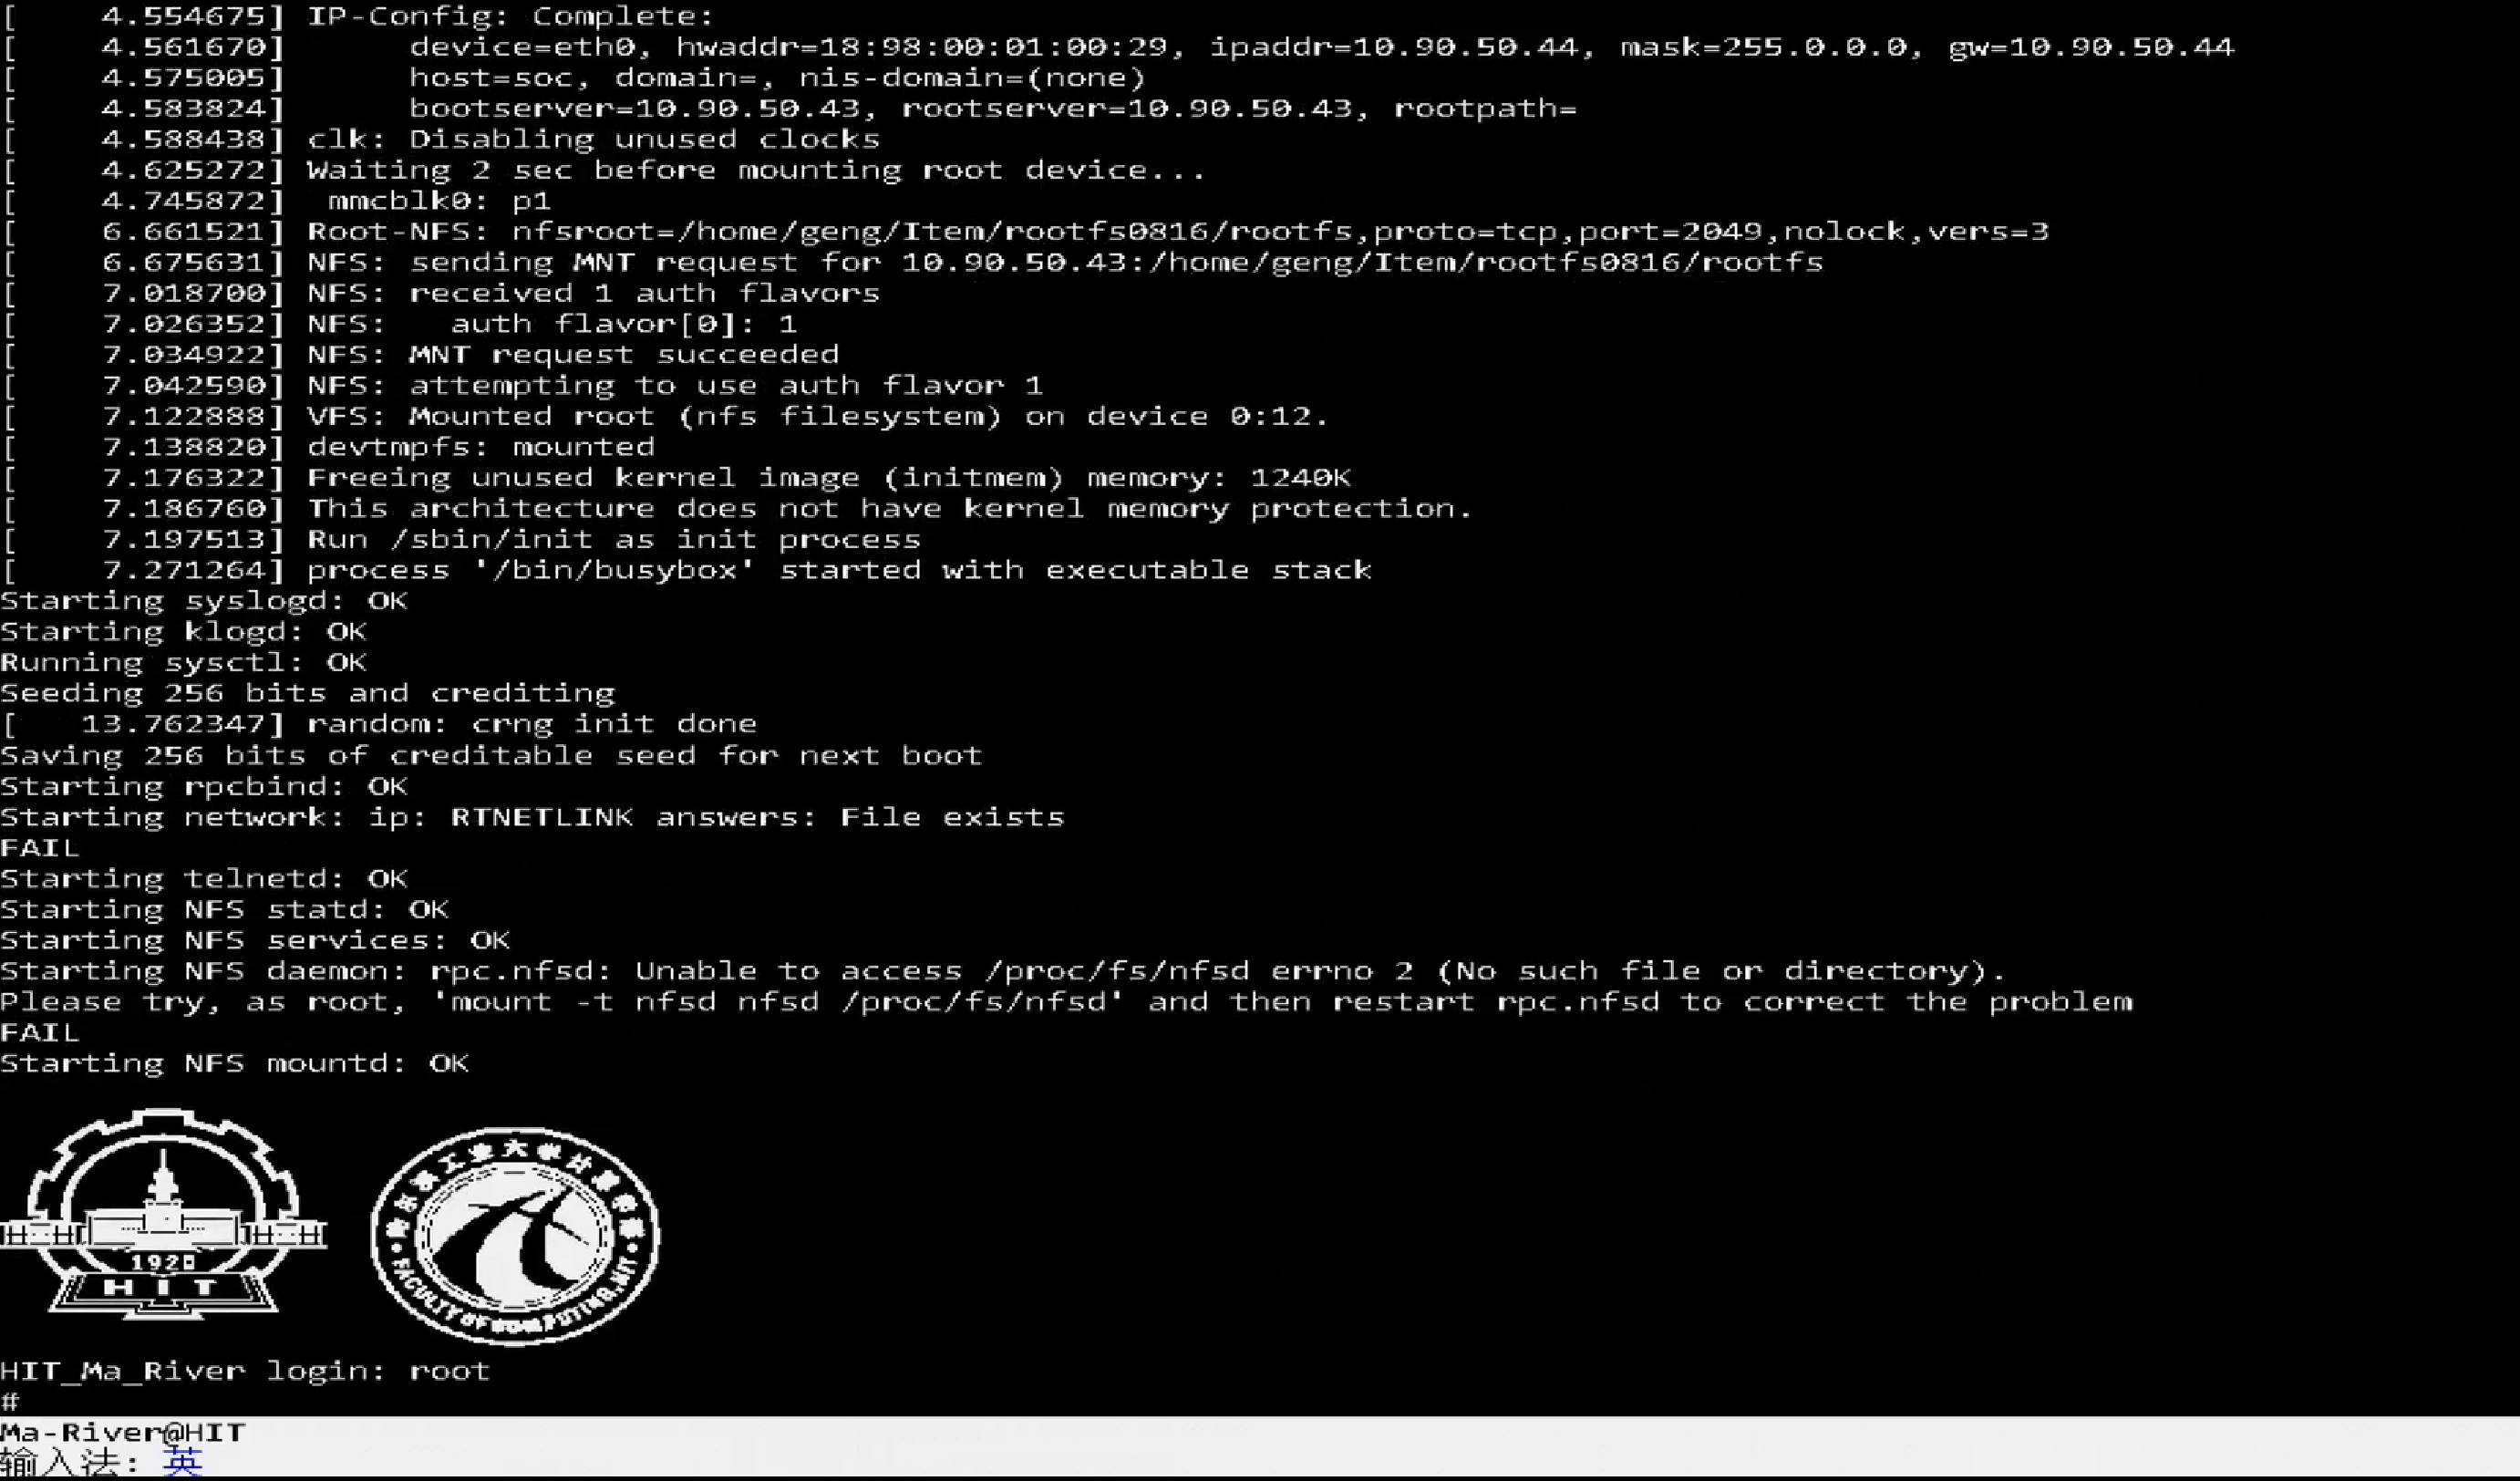
\includegraphics[width=13cm]{img/linux.png}
\caption{Linux启动界面} % 图片标题
\label{pic3} % 图片标签
\end{figure}

\subsubsection{PS/2键盘驱动}
Linux启动后会使用虚拟终端,它的输入最终基于一个完备的input子系统,这给我们自行实现的键盘驱动带来了便利。我们只需要令键盘中断处理程序读取扫描码,通过\texttt{input\_report\_key}向内核的input子系统上报键盘输入事件即可。

\subsubsection{Framebuffer驱动}
为了能够支撑更多GUI应用,我们还为VGA和LCD控制器实现了Framebuffer驱动。Framebuffer驱动的实现包含如下部分:一,开辟一块内存区域,存放每个像素的颜色信息;二,以合适的方式向显示设备传送内存中的颜色信息。
由于我们的VGA控制器和LCD模块本身均采用RGB565颜色格式,故在实现驱动时使用同样的格式进行像素信息的存储,因而每个像素需要2字节空间。
由于我们实现的VGA、LCD控制器均支持DMA,故我们仅需向控制器传送内存区域首地址,由控制器直接进行数据的读取,即可完成图像显示。其中,VGA控制器可自行进行不间断的数据读取;但LCD控制器完成一次数据传输后便会停止,所以我们使用计时器机制,每隔50ms传送一次内存区域首地址,以20Hz刷新率显示图像。

\subsubsection{SD驱动}
由于我们通过AXI QUAD SPI IP核对SD卡进行操作,所以直接使用了该IP核对应的SPI总线驱动;同时,我们也直接使用了Linux内核主线中使用SPI总线的MMC驱动。在设备树中记录设备相关信息后,即可在进入Linux内核后将SD卡分区挂载到目录树中,进行读写操作。

\subsection{用户态组件}
Linux 内核本身并不能提供任何用户态组件,因此我们需要手工编译这一部分。我们选 择了著名的嵌入
式 Linux 开发工具套件 buildroot 来协助完成用户程序的构建。构建过程 中,我们选择了 glibc 作为系统的C/C++ 标准库实现,并使用 busybox 来提供大部分的 命令行工具。由于构建的 rootfs 较大,无法使用
initramfs 等方式直接加载,而 Flash 的读写速度也 较慢并不灵活,因此我们使用 NFS 协议通过网络挂载系
统的根分区。实践证明,在网络稳定的情况下,系统的响应速度并不会受到影响。
我们成功移植了如下内容:
\begin{description}
    \item[GCC] 由于 buildroot 理念在于生成体积更小的根文件系统,所以不支持GCC移植,我们参考linux-from-scratch\footnote{\url{https://www.linuxfromscratch.org/}} 对GCC进行移植,并对glibc以及binutils利用相同方法移植到系统中,此外,由于 Ma-River CPU 实现了FPU,所以在编译时我们添加了支持硬件浮点的选项,经过测试,GCC可以成功编译出浮点指令并成功运行。我们在Ma-River上用移植的GCC编译了小游戏2048,并成功在Ma-River上运行,以此突出我们的移植工作。
    \item[QEMU] 我们成功移植了著名开源项目QEMU,并生成了可以模拟RISC-V架构的系统级模拟器 \text{qemu-system-riscv64} ,但可惜的是实验板内存只有128MB,无法满足系统级模拟器的运行需求。
    \item[Python] 我们移植了Python3,并且添加了数据处理相关的库(numpy,scipy等)。我们还使用Python搭建了简单的http服务器,浏览器可以在局域网中访问板载服务器上的网页。以此证明我们的 CPU 能够在板载资源更充足的情况下运行更加复杂的应用,体现出我们工作的实用性。
    \item[Busybox] 使用Busybox提供大部分命令行工具。
    \item[网络工具] 移植了常用网络工具(ip,ping,wget,nc,ssh)大大提高了后续的移植以及测试工作的效率。
\end{description}

\subsection{新增内容}
\subsubsection{中文支持}
我们在VGA Console和键盘驱动程序的基础上,为Linux终端增加了基本的中文输入输出能力,基于标准的UTF-8编码,不仅可以输入/显示汉字,还可以将文件名等设为中文进行操作。在我们自己实现的CPU及计算机系统上支持中文汉字处理,也是一件颇有意义的事情。

我们的VGA控制器在文本模式下具有二值化图像显示能力,这使得软件理论上可基于字库绘制复杂字符。我们向VGA Console驱动程序中加入了使用Unicode索引的汉字点阵字库(宋体),收录了符合GBK规范的所有汉字。这样驱动程序可在屏幕某位置显示占两格的汉字。我们还对Linux内核中的虚拟终端负责输出字节流解码的部分作出了简要修改,使其不会对汉字对应的UTF-8编码报错,并正确地将汉字对应的Unicode码值传递给底层VGA Console驱动。有趣的是,我们还将哈工大校徽分解为16*16的不同色块存于字库中,映射到Unicode编码中未被汉字使用的区域,这样可以以“显示文本”的方式在屏幕任意位置显示哈工大校徽。
    
对于中文输入,我们自行实现了简单的拼音输入法,它基于Trie树进行查询匹配,支持多字输入、单字选择和简单的拼音分割,操作和普通的拼音输入法类似。我们将VGA文本模式的最下两行供输入法使用,键盘驱动程序在读取到扫描码后,会率先交由输入法模块进行处理,若输入法处于输入状态则拦截这一按键事件,不提交至input子系统。当输入完成后,输入法模块通过\texttt{tty\_insert\_flip\_string}将汉字字符串的UTF-8编码字节流送入虚拟终端的 tty\_port 里。

\subsubsection{GUI应用支持}
我们对LVGL官方演示程序进行了移植,使其能够通过Framebuffer在LCD上输出GUI界面、通过输入子系统读取触摸信息。于是,我们便可以直接通过触摸来操作该演示程序提供的开关等控件,并看到即时的显示反馈。

\subsubsection{GIF动画播放器} 我们实现了一个简单的GIF动画播放器,可以在LCD上显示QQ动态表情等。程序读取指定GIF文件并逐帧解析,使用 LZW压缩算法库 \footnote{\url{https://github.com/jefftime/lzw}} 对像素数据进行解压缩,通过DMA将每帧图像轮番显示在LCD屏幕上,帧率可达20-30FPS。该动画播放器支持通过触摸屏移动图像。
\subsubsection{3D模型实时渲染} 
由于Ma-River CPU具有完备的浮点运算能力,并且我们的LCD控制器支持DMA加速绘制,这使得我们可以实现一些较复杂的图形学应用,例如3D模型渲染。

我们使用C语言编写了一个简单3D模型软渲染器(只使用纯CPU指令),使用Blender建立较复杂的3D模型,将其三角面信息以stl格式导出,渲染器据此得出模型顶点的三维坐标,将其乘以视图矩阵和投影矩阵进行投影变换(这需要大量浮点运算),投影到二维平面上,再绘制顶点间的线条,通过DMA将其显示到LCD屏幕上。我们的软渲染器是动态实时的,在Linux下运行时帧率可达12FPS左右,视角可自动随物体转动,也支持通过触摸移动视角,具有很好的交互性。
% Part 5 致谢
\chapter*{附录}
\appendix
\renewcommand{\appendixname}{Appendix~\Alph{section}}
\section*{致谢}

\quad 我们对以下团体或个人表示由衷的感谢,没有他们,马家沟河项目是无法走到今天的。

\begin{itemize}
    \item 感谢龙芯中科提供的设备与比赛平台支持,衷心祝愿他们能够在国产CPU道路上越走越远。
    \item 感谢舒燕君和刘国军两位指导老师的帮助、指导和关心。
    \item 感谢胡光辉等隔壁团队同学们的无私帮助。
    \item 感谢张清钰、王永琪、郑翔宇、丛日东等学长的帮助。
    \item 感谢清华大学ZenCove、NonTrivalMips、重庆大学CDIM等往届团队,他们开源的往届作品及经验分享对我们的工作起到了极大帮助和启发作用。
    \item 感谢姚永斌老师的《超标量处理器设计》一书,此书给予了我们很大启发,没有它就没有Ma-River现在的微架构设计。
\end{itemize}

\section*{参考资料}

\quad 本项目参考了包括但不限于下列书籍、资料、网站或开源项目:

\begin{itemize}
    \item 姚永斌. 超标量处理器设计[M]. 清华大学出版社: 201404.
    \item 唐朔飞. 计算机组成原理(第三版)[M]. 哈尔滨工业大学出版社: 202010.
    \item 汪文祥,邢金璋. CPU设计实战[M]. 机械工业出版社: 202101.
    \item CEMU文档:\url{http://cemu.cyyself.name/}
    \item CDIM项目:\url{https://github.com/Maxpicca-Li/CDIM}
    \item ZenCove项目:\url{https://github.com/zencove-thu/}
    \item NonTrivalMips项目:\url{https://github.com/trivialmips/nontrivial-mips}
    \item SHIT Core项目:\url{https://github.com/Superscalar-HIT-Core/Superscalar-HIT-Core-NSCSCC2020}
    \item TinyVGA:\url{http://tinyvga.com/}
    \item Framebuffer\_driver\_rpi:\url{https://github.com/dsoastro/framebuffer_driver_rpi}
\end{itemize}

\end{document}